\documentclass{article}
\usepackage[utf8]{inputenc}
\usepackage{amsmath}
\usepackage{pdfpages}
\usepackage{booktabs}
\usepackage{hyperref}
\usepackage{enumitem}
\usepackage{url}
\usepackage{endnotes}
\usepackage[utf8]{inputenc}
\usepackage{graphicx}
\usepackage{subcaption}
\usepackage[numbers]{natbib}
\graphicspath{ {figures/} }
\usepackage{array}
\begin{document}
\title{Highway Corridor Modeling}
\author{Bingyi Fan & Yingying Chen \\ \bigskip University of California, Berkeley}
\date{May 2019}

\maketitle
\newpage
\tableofcontents

%%%%%%%%%%%%%%%%%%%%%%%%%%%%%%%%%%%%%%%
% Abstract
%%%%%%%%%%%%%%%%%%%%%%%%%%%%%%%%%%%%%%%
\newpage
\section{Abstract}
In this project, we analyzed existing operating conditions of a typical freeway section, then developed and evaluated control and operational improvements for the section. The analysis was performed with computer simulation techniques.

\section{Introduction}
The goal of this project is to: \begin{enumerate}
    \item simulate the real bottlenecks and congestion on the studied highway section in AIMSUN, a computer traffic simulation program.
    \item study the impacts of potential traffic growth on the current highway operations.
    \item experiment and analyze potential approaches to mitigate congestion under both normal and increased demands.
    \item suggest the best approach that can be used to improve the highway.
\end{enumerate}

We will mainly use speed as shown in time-space diagrams as the indicator of highway operational efficiency. Other metrics we consider include average and total travel time and delay.

%%%%%%%%%%%%%%%%%%%%%%%%%%%%%%%%%%%%%%%
% Introduction
%%%%%%%%%%%%%%%%%%%%%%%%%%%%%%%%%%%%%%%
\section{Method}
The study section has a total of 8.83 miles. We divided it into 19 subsections for study purposes. There are three travel lanes with auxiliary lanes in certain segments of the freeway. A total of nine on-and off-ramps are in this section. The observed free-flow speed is 65 mph and the capacity is 2,000 vph/lane. 
\bigskip

Figure \ref{fig:time-space_old} is a contour plot of the existing operating conditions in the study section during a three hour PM peak period (3:30 to 6:45 pm). There are thirteen 15-minute analysis periods. Green indicates that demand is less than the freeway capacity, yellow indicates the location of active bottlenecks, and red indicates congestion (queues upstream of a bottleneck). 
\begin{figure}[!htbp]
    \centering
    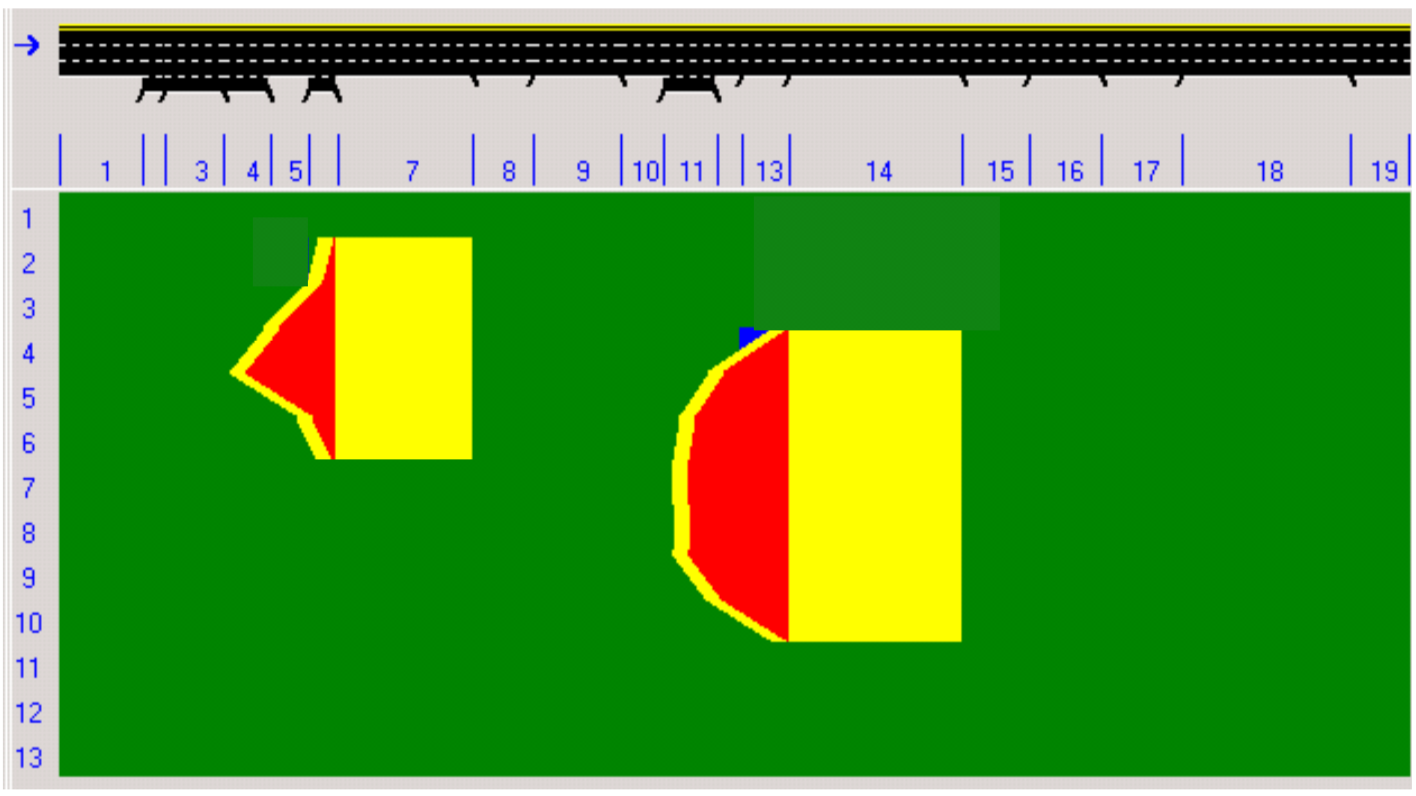
\includegraphics[width=12cm]{time_space_old.png}
    \caption{Study Section Empirical Evidence}
    \label{fig:time-space_old}
\end{figure}


%%%%%%%%%%%%%%%%%%%%%%%%%%%%%%%%%%%%%%%
% Methodology
%%%%%%%%%%%%%%%%%%%%%%%%%%%%%%%%%%%%%%%
\subsection{Model Operational}
First, we performed a baseline model run with the input data file, and compared the model predicted performance with the existing conditions.
\begin{figure}
    \centering
    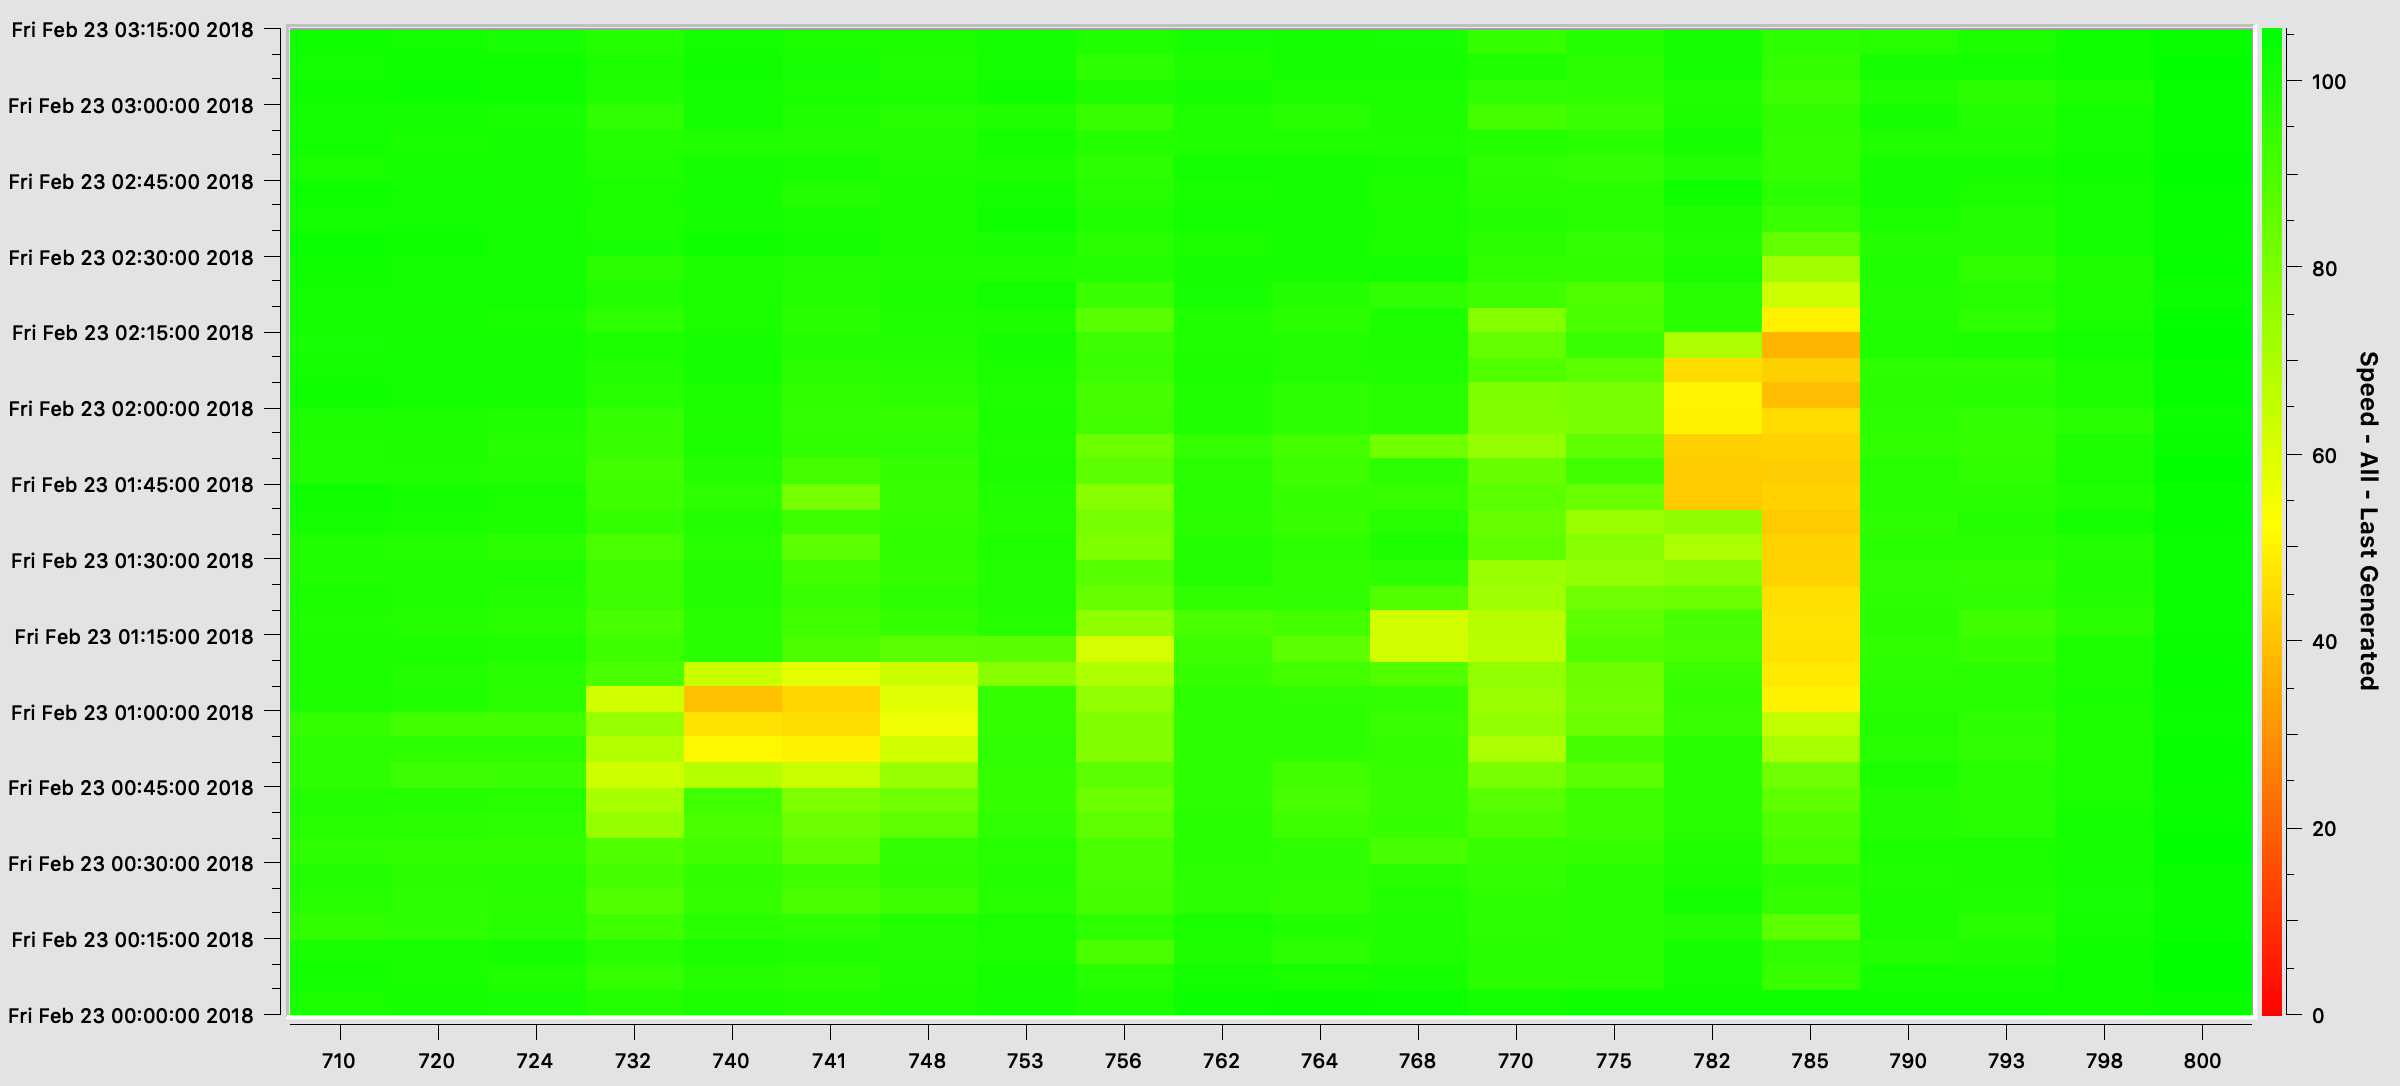
\includegraphics[width=12cm]{original.png}
    \caption{Time-space diagram of baseline model run}
    \label{fig:time-space}
\end{figure}
As shown in Figure \ref{fig:time-space}, vehicles are travelling with free flow speed for the most of study period. However, in Figure \ref{fig:time-space_old}, it is easy to observe two bottlenecks/congestion area at study section 4-7 and section 11-14. Comparing with the existing operating conditions, traffic condition in the baseline model is not accurate. Therefore, calibration should be applied to correct the model.


\subsection{Model Verification/Calibration}
After the baseline model run, we calibrated the model parameters as appropriate based on the empirical evidence shown in Figure \ref{fig:time-space_old}. Figure \ref{fig:congested_1} is the time-space diagram of speed contours after the calibration. 

\begin{figure}[!htbp]
    \centering
    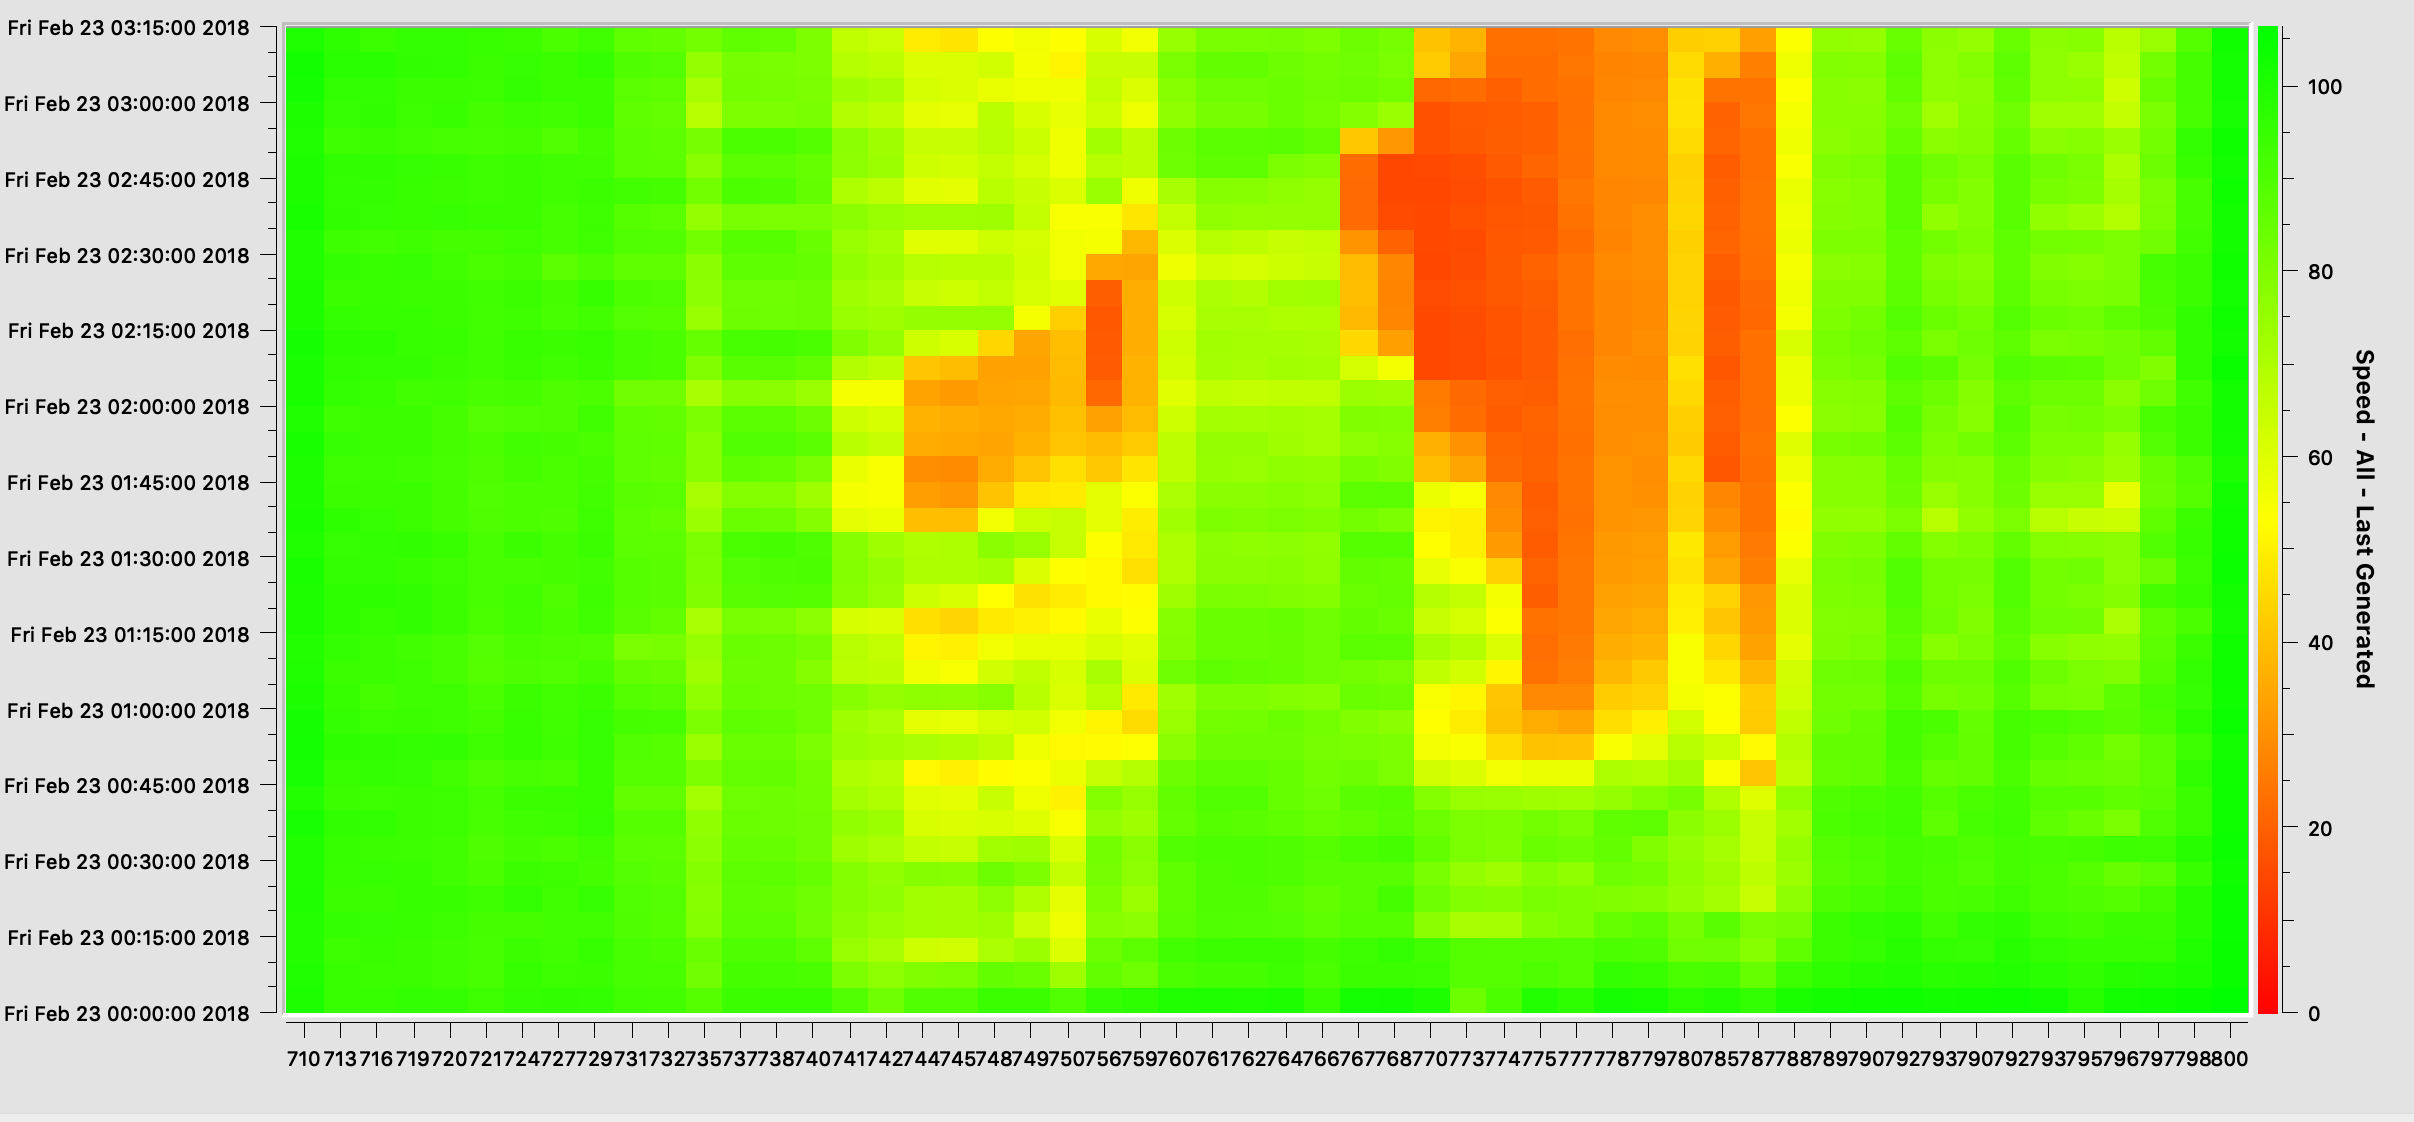
\includegraphics[width=12cm]{congested.png}
    \caption{Time-space diagram after calibration}
    \label{fig:congested_1}
\end{figure}

We modified the parameters such as acceleration and deceleration of cars as well as parameters in the car following model. As shown in Figure \ref{fig:car_param} are parameters of the vehicle model after our calibration. For the car-following sensitivity factor, we utilized results from two sources, where El Khoury and Hobeika proposed a range of 1.6 for timid drivers and 0.3 for aggressive drivers \cite{El}, and Soria proposed values from 1.25 for the timid drivers to 0.35 for the aggressive drivers \cite{Soria}. According to Soria, time gap is equivalent to or greater than reaction time, thus we set the gap to be 2.0 seconds with a 1.0 deviation \cite{hdm}. We also favor stop and go driving behaviors, which are commonly seen on congested highways.

The highway operational metrics are summarized in Table \ref{basic}.

\begin{figure}[!htbp]
    \centering
    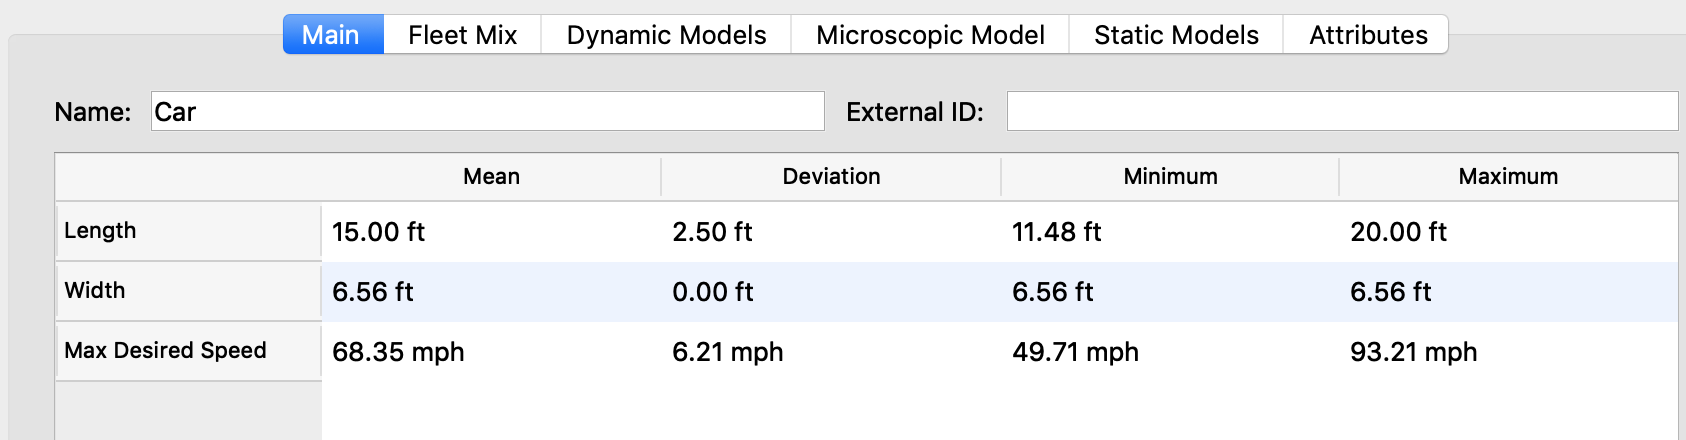
\includegraphics[width=12cm]{car_param.png}
    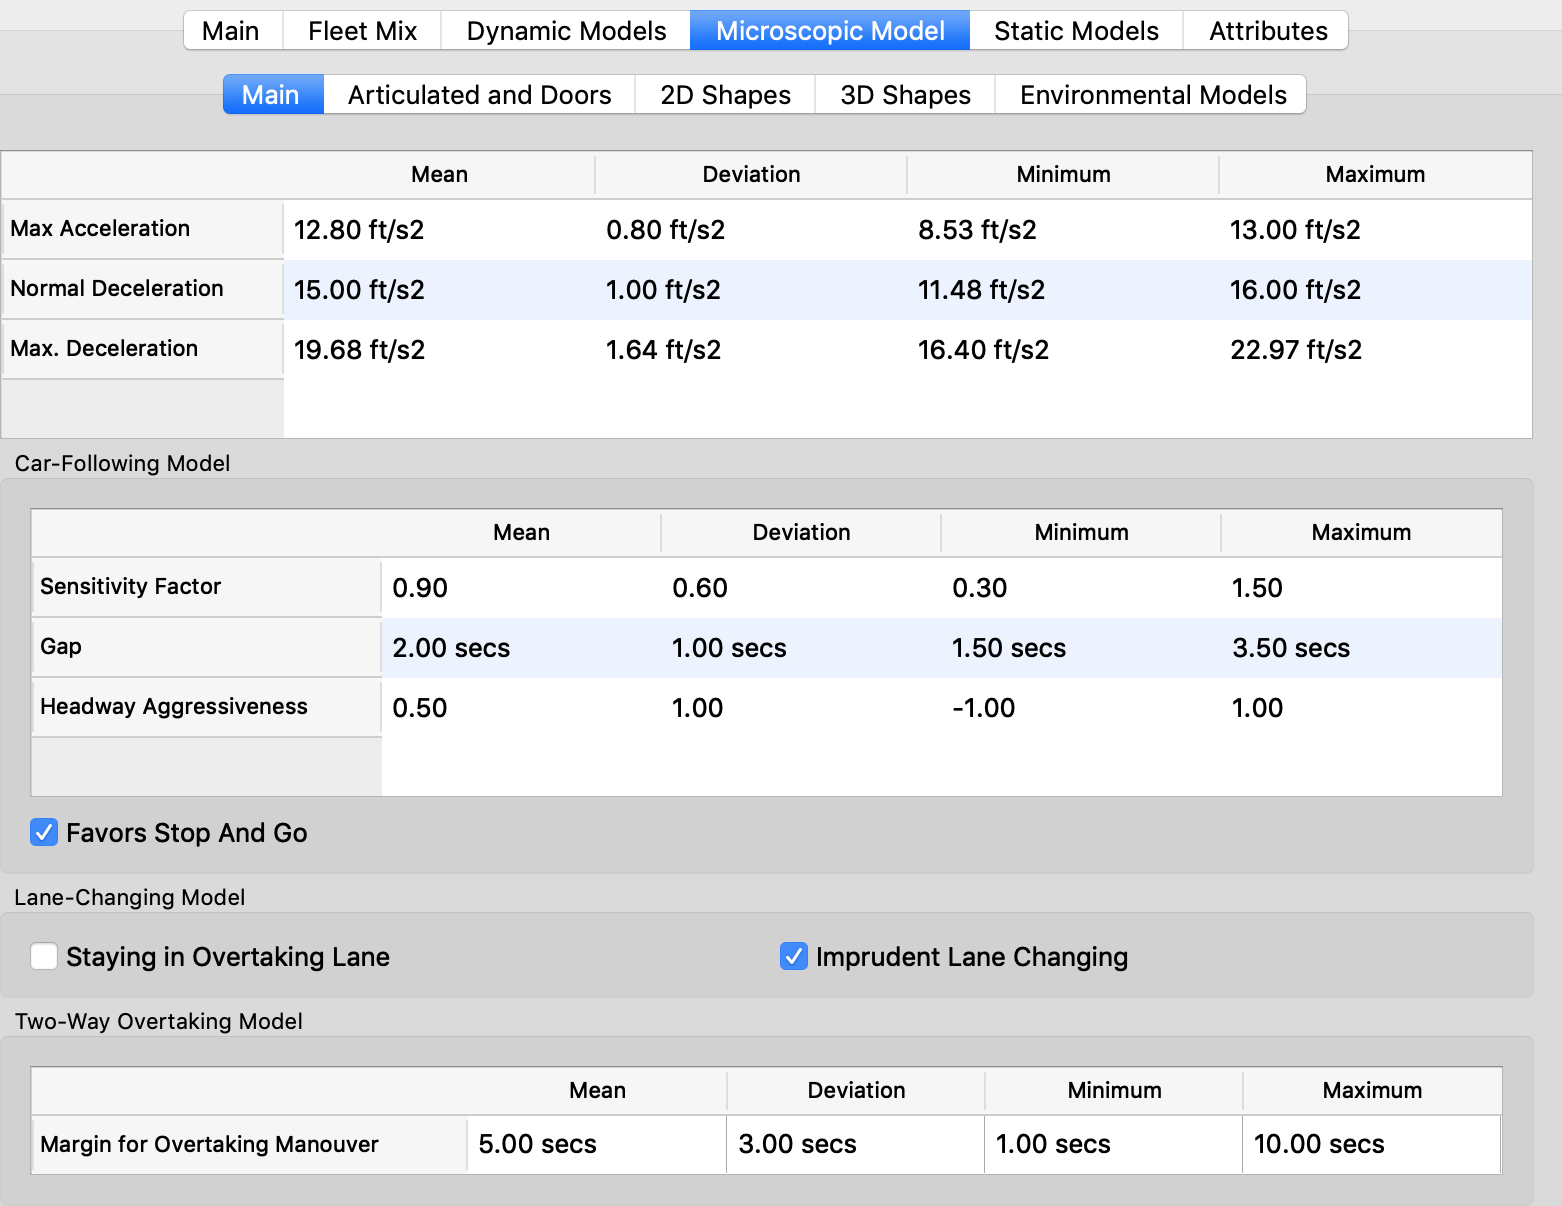
\includegraphics[width=12cm]{car_model.png}
    \caption{Parameters of the vehicle model after calibration}
    \label{fig:car_param}
\end{figure}

% 	Time Series	Value	Standard Deviation	Units
% 	Delay Time - Car	43.75	32.27	sec/mi
% 	Density - Car	38.06	N/A	veh/mi
% 	Flow - Car	8265.85	N/A	veh/h
% 	Harmonic Speed - Car	36.58	10.86	mph
% 	Input Count - Car	28121	N/A	veh
% 	Input Flow - Car	8652.62	N/A	veh/h
% 	Max. Virtual Queue - Car	1533	N/A	veh
% 	Mean Queue - Car	20.50	N/A	veh
% 	Mean Virtual Queue - Car	1097.65	N/A	veh
% 	Missed Turns - Car	42	N/A	
% 	Number of Lane Changes - Car	7795.33	N/A	#/mi
% 	Number of Stops - Car	0	N/A	#/veh/mi
% 	Speed - Car	39.80	10.78	mph
% 	Stop Time - Car	1.94	6.66	sec/mi
% 	Total Number of Lane Changes - Car	242402	N/A	
% 	Total Number of Stops - Car	4931.85	N/A	
% 	Total Travel Time - Car	3722.62	N/A	h
% 	Total Travel Time (Vehicles Inside) - All	83.74	N/A	h
% 	Total Travel Time (Vehicles Inside) - Car	83.74	N/A	h
% 	Total Travel Time (Waiting Out) - All	82.43	N/A	h
% 	Total Travel Time (Waiting Out) - Car	82.43	N/A	h
% 	Total Travelled Distance - Car	132591.65	N/A	mi
% 	Total Travelled Distance (Vehicles Inside) - All	4395.35	N/A	mi
% 	Total Travelled Distance (Vehicles Inside) - Car	4395.35	N/A	mi
% 	Travel Time - Car	98.42	31.48	sec/mi
% 	Vehicles Inside - Car	1257	N/A	veh
% 	Vehicles Lost Inside - Car	0	N/A	veh
% 	Vehicles Lost Outside - Car	0	N/A	veh
% 	Vehicles Outside - Car	26864	N/A	veh
% 	Vehicles Waiting to Enter - Car	1070	N/A	veh
% 	Waiting Time Virtual Queue - Car	410.20	746.17	sec

\begin{table}[]
\centering
\caption{Metrics of Calibrated Model}
\begin{tabular}{|l|l|}
\hline
Flow (vph)                    & 8266.85 \\ \hline
Total delay (hr)              & 887.02  \\ \hline
Average delay (sec/veh)       & 386.31  \\ \hline
Average travel time (sec/veh) & 476.56  \\ \hline
\end{tabular}
\label{basic}
\end{table}

\section{Experiments and Results}
In this section, we will discuss analysis performed using the AIMSUN microscopic simulation model in details.

\subsection{Impacts of Traffic Growth}
We evaluated the impact of increases in the total traffic demand in the study corridor for 120\% of the existing demand in 5\% increments.

%110 	Time Series	Value	Standard Deviation	Units
% 	Delay Time - Car	68.98	49.97	sec/mi
% 	Density - Car	50.79	N/A	veh/mi
% 	Flow - Car	8450.46	N/A	veh/h
% 	Harmonic Speed - Car	29.13	11.76	mph
% 	Input Count - Car	29549	N/A	veh
% 	Input Flow - Car	9092	N/A	veh/h
% 	Max. Virtual Queue - Car	2850	N/A	veh
% 	Mean Queue - Car	72.09	N/A	veh
% 	Mean Virtual Queue - Car	1947.98	N/A	veh
% 	Missed Turns - Car	31	N/A	
% 	Number of Lane Changes - Car	8699.73	N/A	#/mi
% 	Number of Stops - Car	0.02	N/A	#/veh/mi
% 	Speed - Car	33.88	12.67	mph
% 	Stop Time - Car	5.73	11.52	sec/mi
% 	Total Number of Lane Changes - Car	270525	N/A	
% 	Total Number of Stops - Car	15751.87	N/A	
% 	Total Travel Time - Car	4780.57	N/A	h
% 	Total Travel Time (Vehicles Inside) - All	155.63	N/A	h
% 	Total Travel Time (Vehicles Inside) - Car	155.63	N/A	h
% 	Total Travel Time (Waiting Out) - All	217.81	N/A	h
% 	Total Travel Time (Waiting Out) - Car	217.81	N/A	h
% 	Total Travelled Distance - Car	133853.26	N/A	mi
% 	Total Travelled Distance (Vehicles Inside) - All	6869.99	N/A	mi
% 	Total Travelled Distance (Vehicles Inside) - Car	6869.99	N/A	mi
% 	Travel Time - Car	123.58	49.35	sec/mi
% 	Vehicles Inside - Car	2085	N/A	veh
% 	Vehicles Lost Inside - Car	0	N/A	veh
% 	Vehicles Lost Outside - Car	0	N/A	veh
% 	Vehicles Outside - Car	27464	N/A	veh
% 	Vehicles Waiting to Enter - Car	2722	N/A	veh
% 	Waiting Time Virtual Queue - Car	554.96	1064.50	sec


%120 	Time Series	Value	Standard Deviation	Units
% 	Delay Time - Car	111.88	92.84	sec/mi
% 	Density - Car	69.17	N/A	veh/mi
% 	Flow - Car	8464.31	N/A	veh/h
% 	Harmonic Speed - Car	21.59	12.06	mph
% 	Input Count - Car	30845	N/A	veh
% 	Input Flow - Car	9490.77	N/A	veh/h
% 	Max. Virtual Queue - Car	4645	N/A	veh
% 	Mean Queue - Car	310.82	N/A	veh
% 	Mean Virtual Queue - Car	2843.05	N/A	veh
% 	Missed Turns - Car	28	N/A	
% 	Number of Lane Changes - Car	8466.07	N/A	#/mi
% 	Number of Stops - Car	0.06	N/A	#/veh/mi
% 	Speed - Car	28.32	13.91	mph
% 	Stop Time - Car	23.46	47.77	sec/mi
% 	Total Number of Lane Changes - Car	263259	N/A	
% 	Total Number of Stops - Car	55021.96	N/A	
% 	Total Travel Time - Car	6121.53	N/A	h
% 	Total Travel Time (Vehicles Inside) - All	263.32	N/A	h
% 	Total Travel Time (Vehicles Inside) - Car	263.32	N/A	h
% 	Total Travel Time (Waiting Out) - All	373.32	N/A	h
% 	Total Travel Time (Waiting Out) - Car	373.32	N/A	h
% 	Total Travelled Distance - Car	131040.09	N/A	mi
% 	Total Travelled Distance (Vehicles Inside) - All	8095.72	N/A	mi
% 	Total Travelled Distance (Vehicles Inside) - Car	8095.72	N/A	mi
% 	Travel Time - Car	166.73	92.95	sec/mi
% 	Vehicles Inside - Car	3336	N/A	veh
% 	Vehicles Lost Inside - Car	0	N/A	veh
% 	Vehicles Lost Outside - Car	0	N/A	veh
% 	Vehicles Outside - Car	27509	N/A	veh
% 	Vehicles Waiting to Enter - Car	4633	N/A	veh
% 	Waiting Time Virtual Queue - Car	569.57	1195.13	sec


\begin{itemize}
\item {Result for 5\% increase}
\newline
As shown in Figure \ref{fig:increase_05}, the two bottlenecks share a very similar pattern as the calibrated result. With a closer observation, we can find that congested area became larger with the 5\% demand increase. The metrics are summarized in Table \ref{5per}.
\begin{figure}
    \centering
    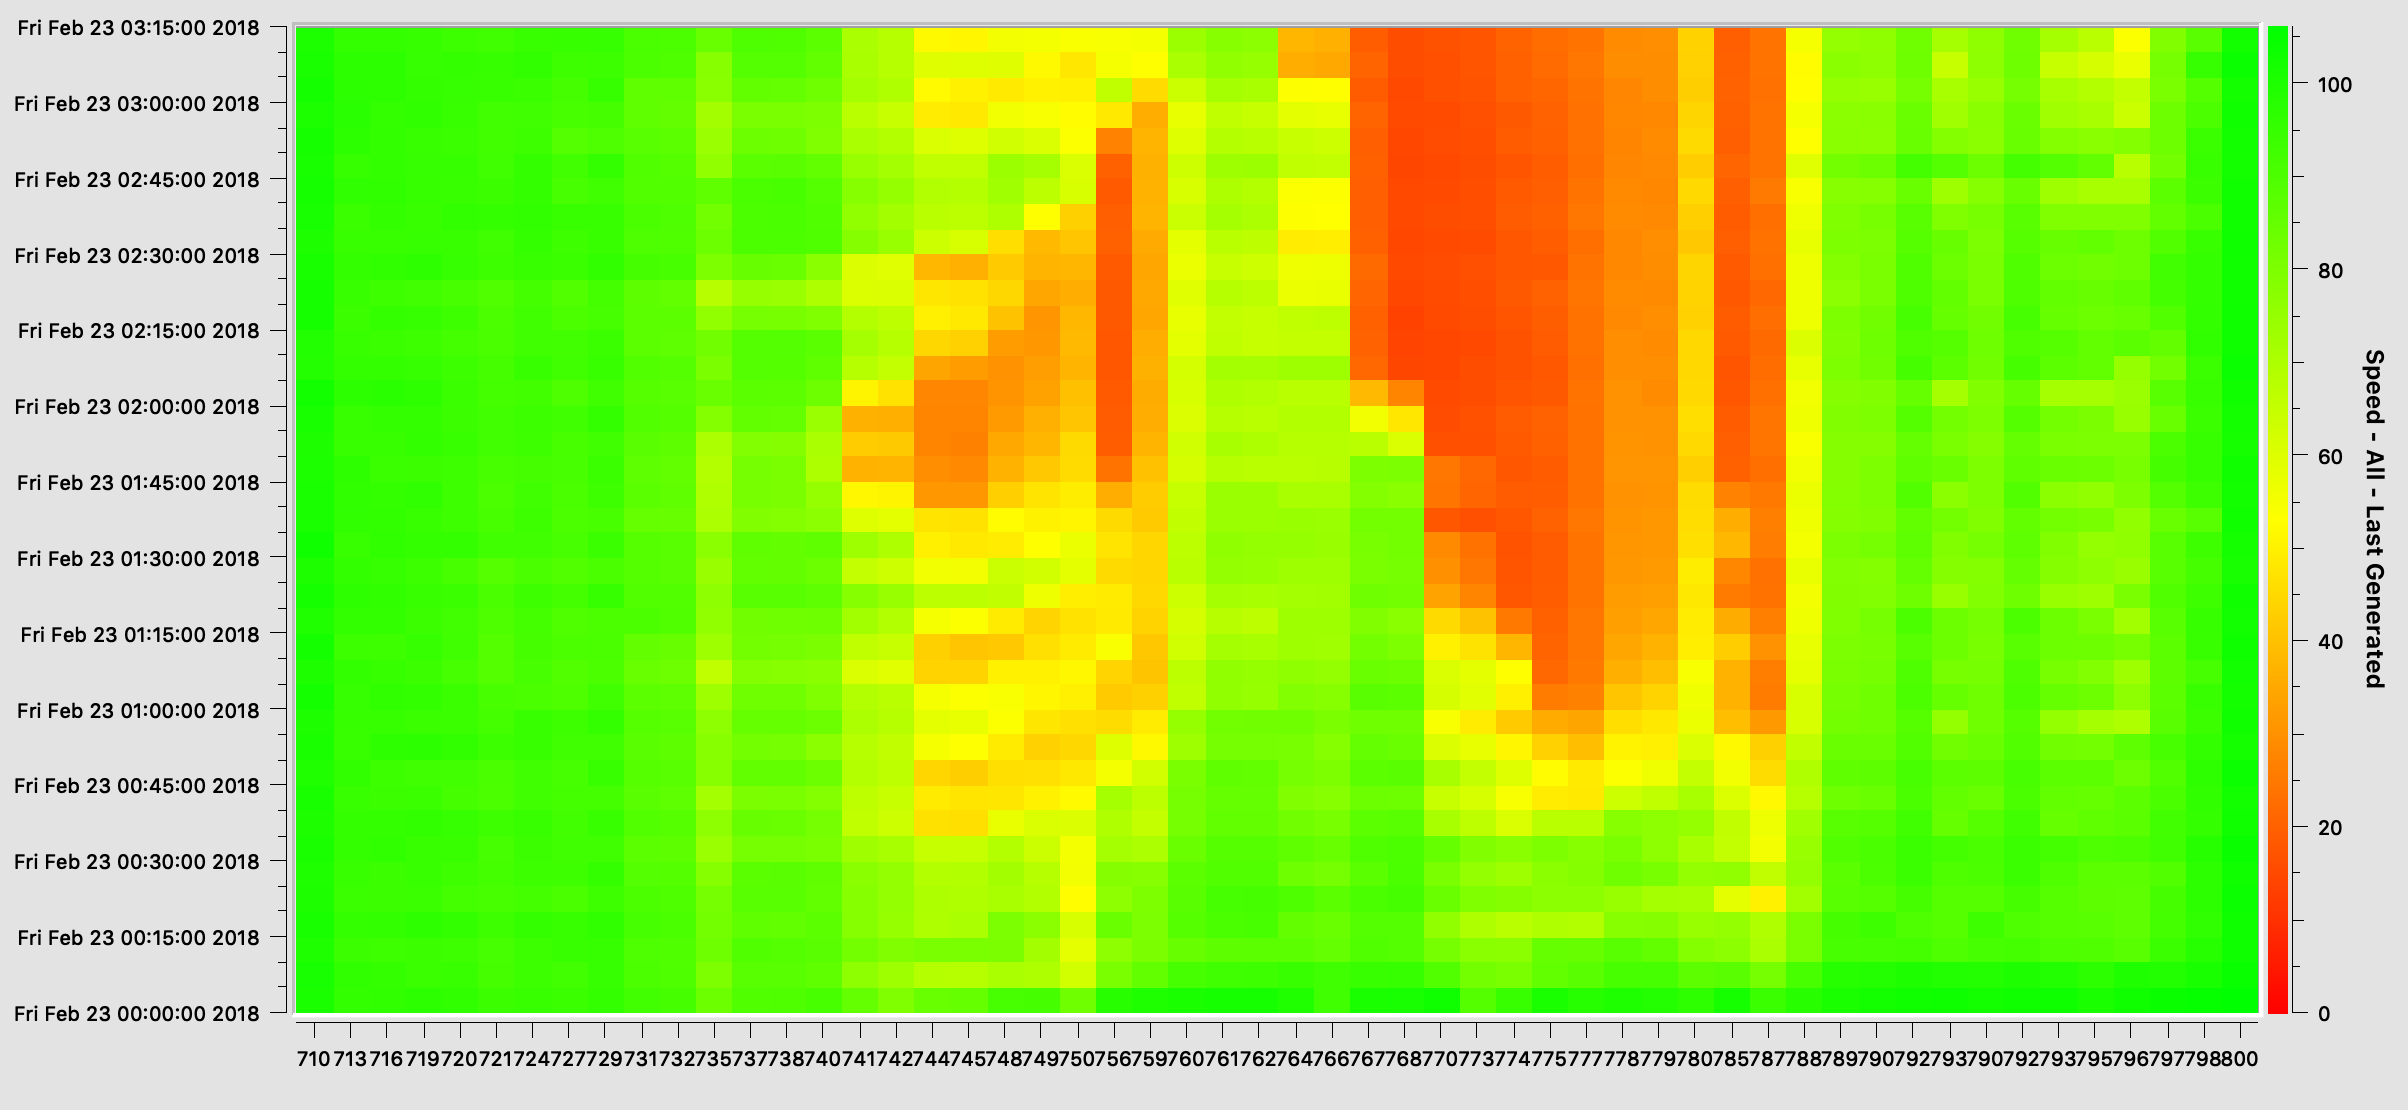
\includegraphics[width=12cm]{increase_05.png}
    \caption{Time-space diagram for simulation with 5\% demand increase}
    \label{fig:increase_05}
\end{figure}

\begin{table}[]
\centering
\caption{Matrics for 5\% Demand Increase}
\begin{tabular}{|l|l|}
\hline
Flow (vph)                    & 8365.32 \\ \hline
Total delay (hr)              & 1204.65 \\ \hline
Average delay (sec/veh)       & 512.96  \\ \hline
Average travel time (sec/veh) & 520.37  \\ \hline
\end{tabular}
\label{5per}
\end{table}


\item {Result for 10\% increase}
\newline
As the total demand increases by 10\%, traffic became much worse as shown in Figure \ref{fig:increase_10}, where the two bottlenecks were connected together. The metrics are summarized in Table \ref{10per}.
\begin{figure}
    \centering
    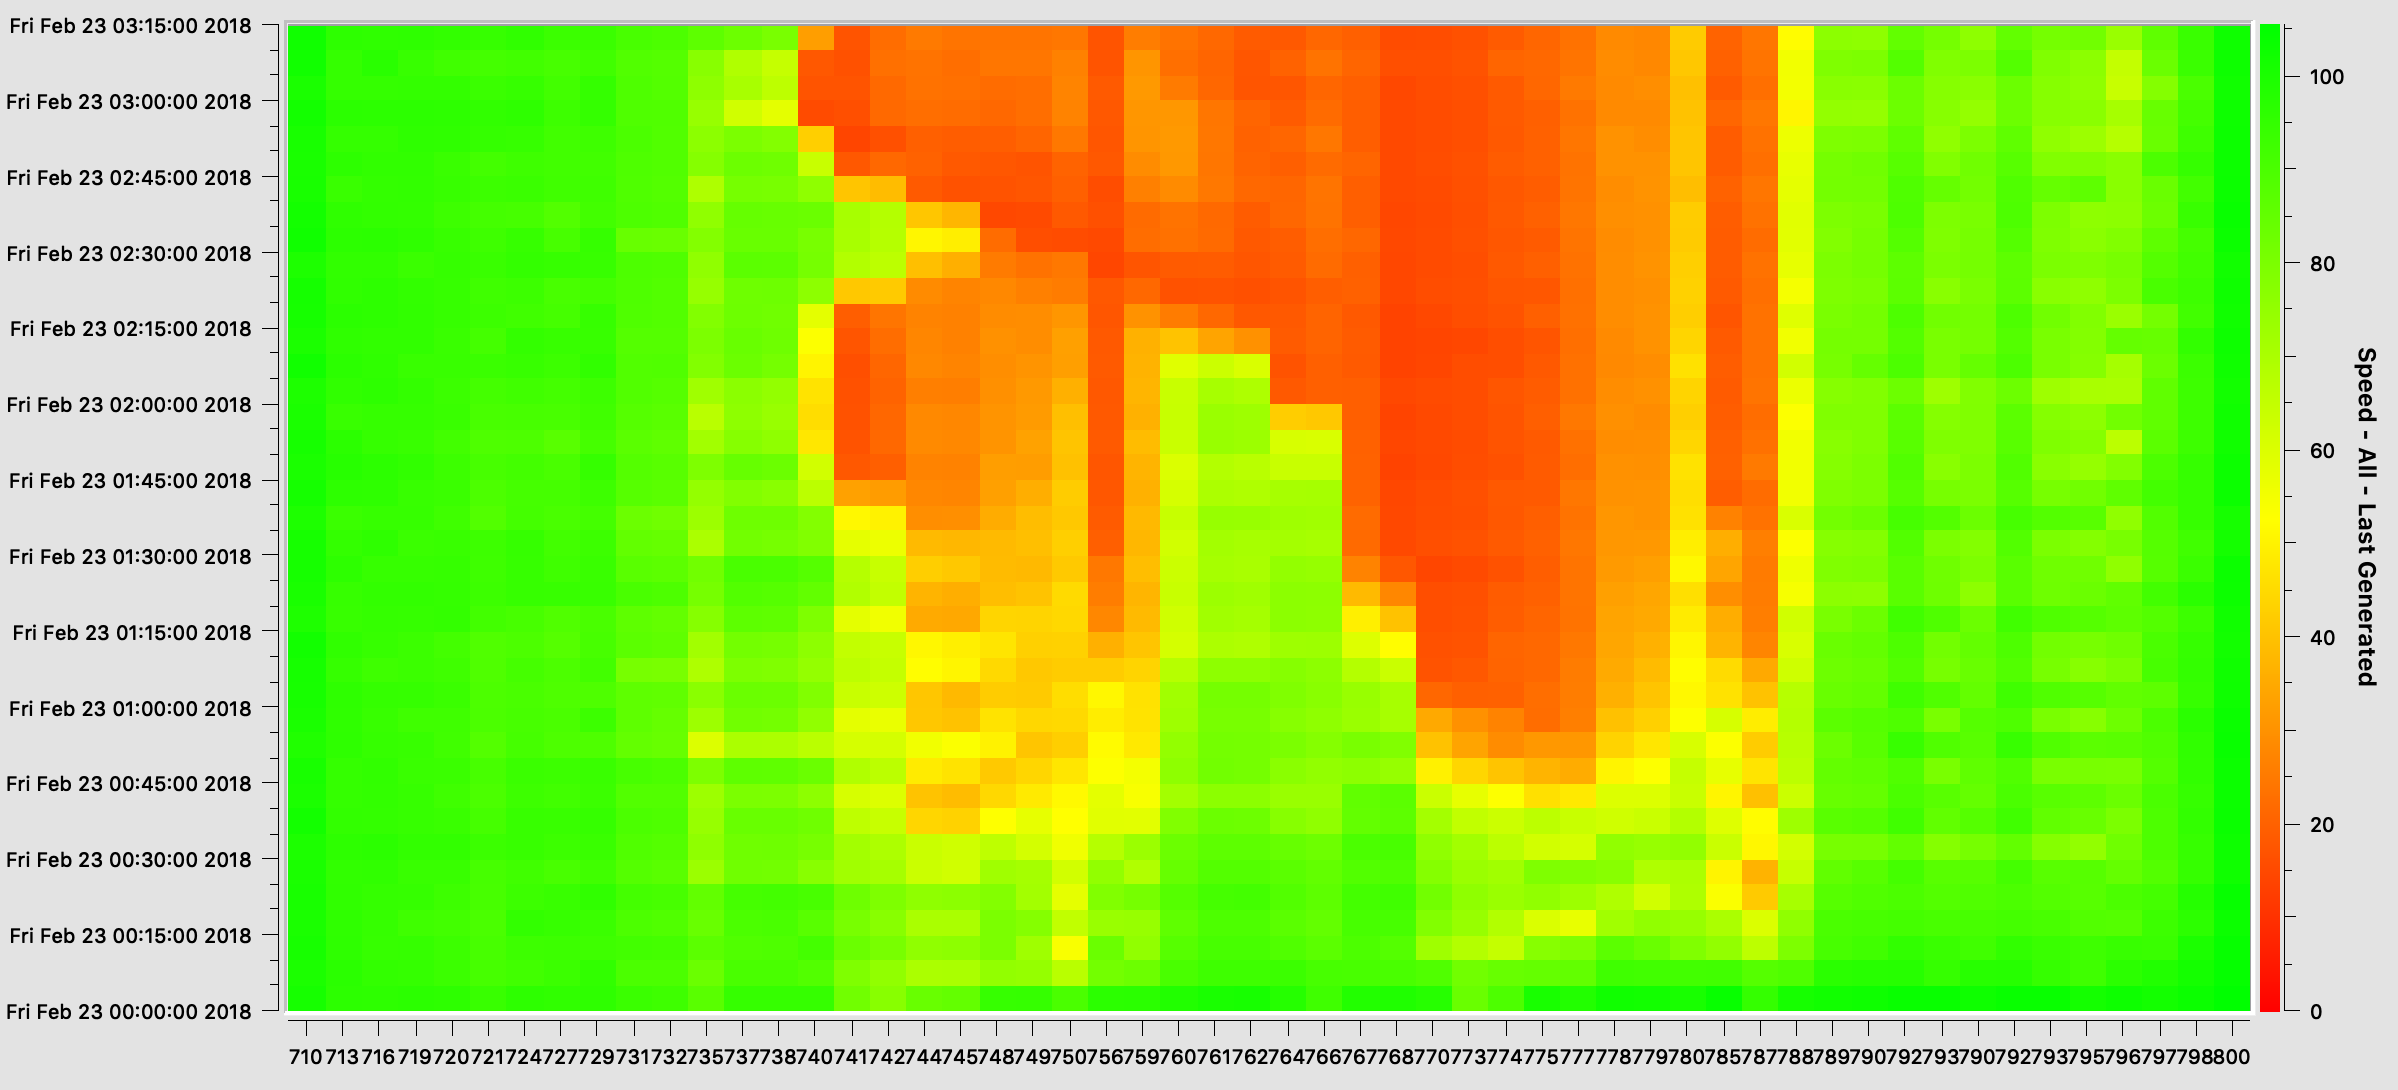
\includegraphics[width=12cm]{increase_10.png}
    \caption{Time-space diagram for simulation with 10\% demand increase}
    \label{fig:increase_10}
\end{figure}

\begin{table}[]
\centering
\caption{Matrics for 10\% Demand Increase}
\begin{tabular}{|l|l|}
\hline
Flow (vph)                    & 8450.46 \\ \hline
Total delay (hr)              & 1429.76 \\ \hline
Average delay (sec/veh)       & 609.09  \\ \hline
Average travel time (sec/veh) & 582.42  \\ \hline
\end{tabular}
\label{10per}
\end{table}


\item {Result for 15\% increase}
\newline
Figure \ref{fig:increase_15} shows the speed contour result for a 15\% increase. With a 15\% increase in total demand, the downstream bottleneck developed much further as compared to Figure \ref{fig:increase_10} while the upstream bottleneck does not share a drastic change. This is because queue from the first bottleneck propagated to the second bottleneck, causing situations at the second bottleneck to be worse. The metrics are summarized in Table \ref{15per}.
\begin{figure}
    \centering
    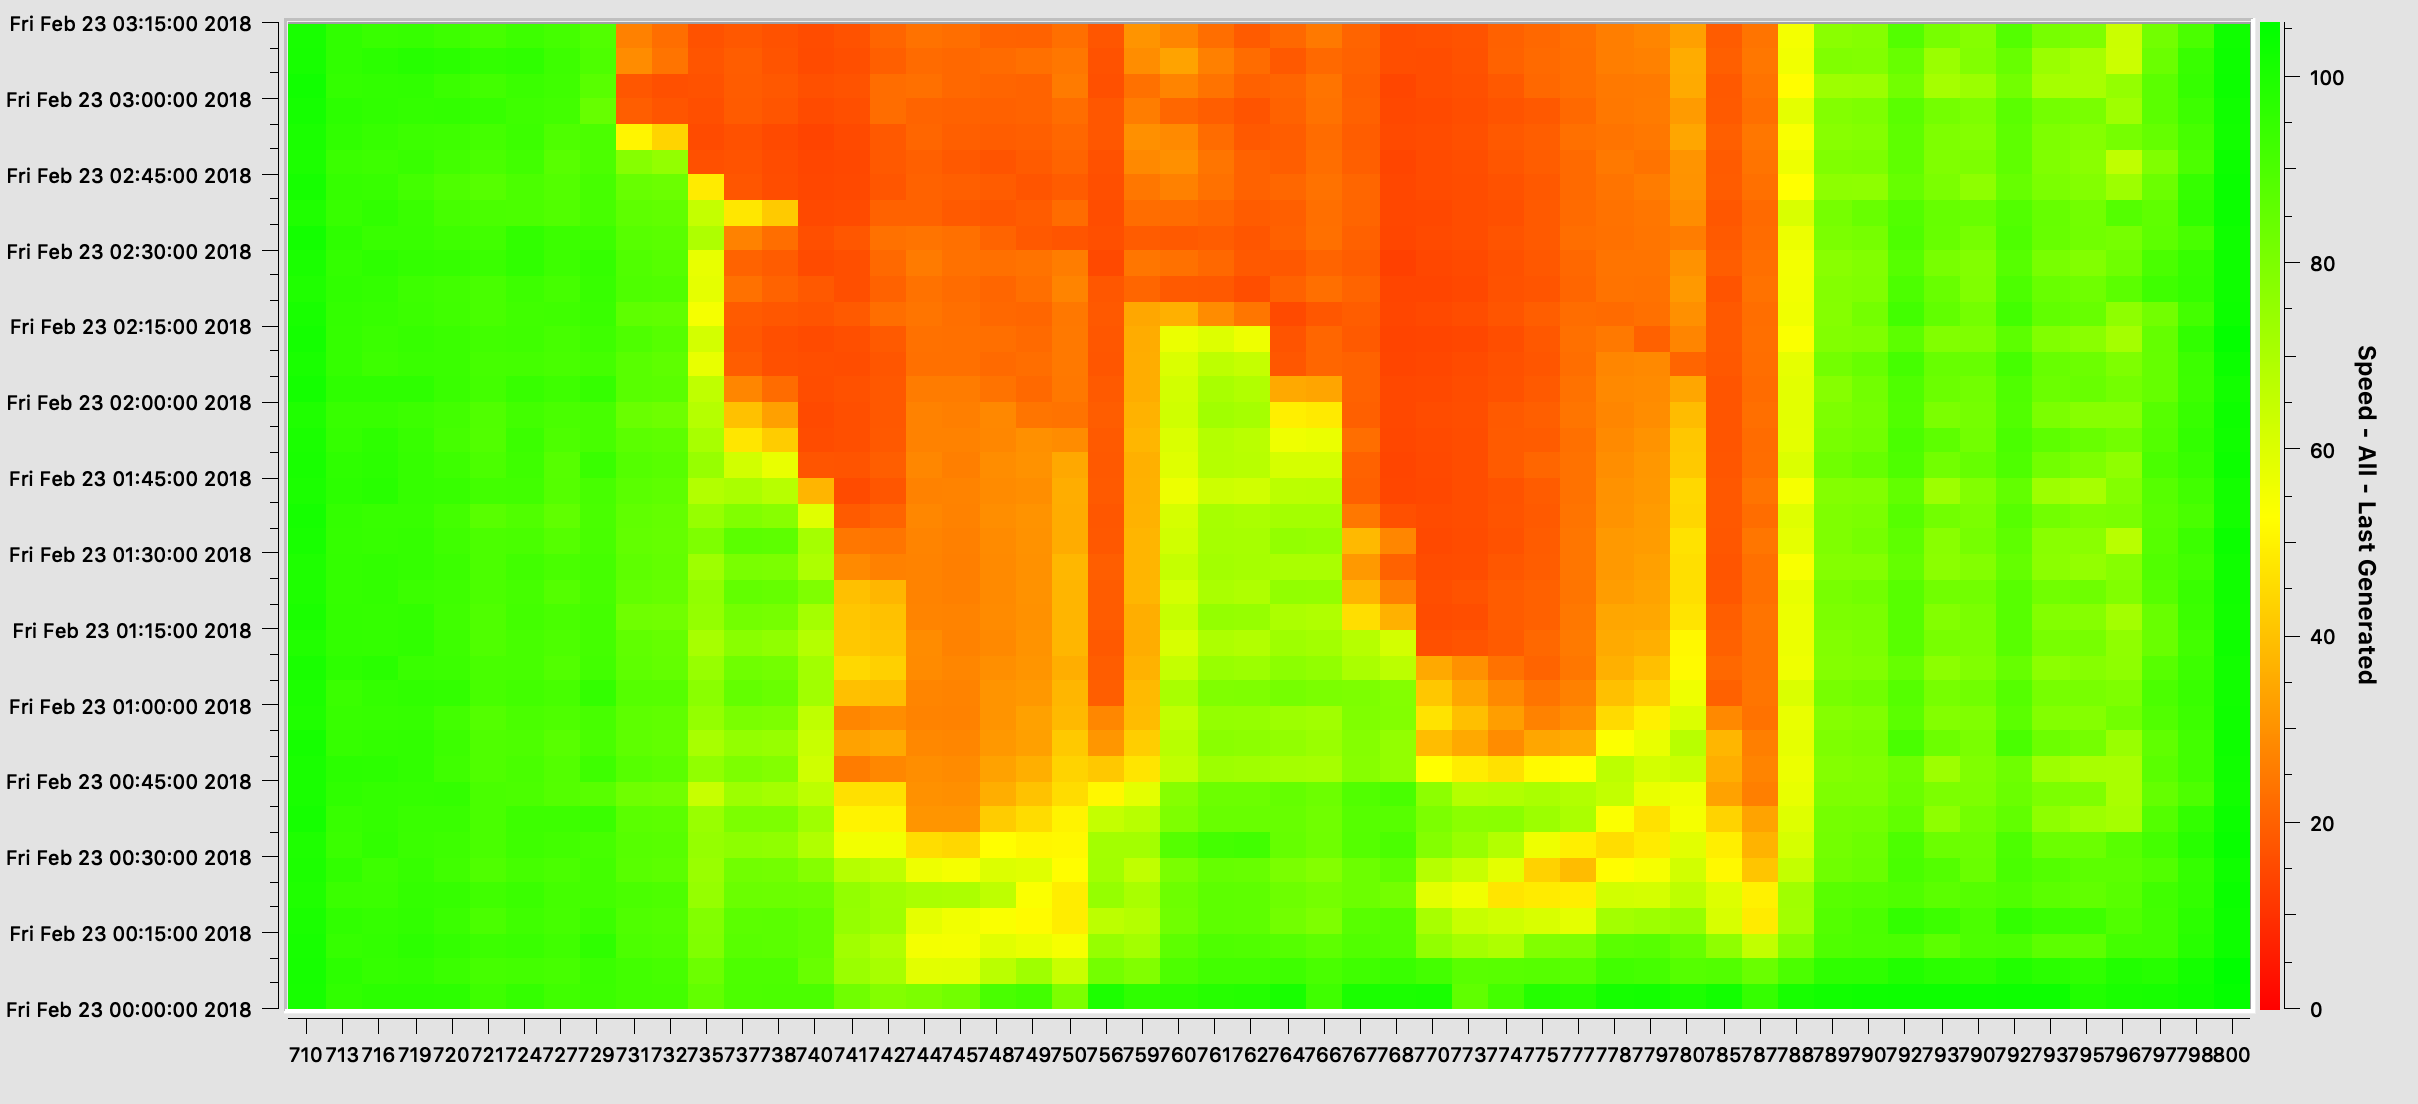
\includegraphics[width=12cm]{increase_15.png}
    \caption{Time-space diagram for simulation with 15\% demand increase}
    \label{fig:increase_15}
\end{figure}

\begin{table}[]
\centering
\caption{Matrics for 15\% Demand Increase}
\begin{tabular}{|l|l|}
\hline
Flow (vph)                    & 8458.98 \\ \hline
Total delay (hr)              & 1789.58 \\ \hline
Average delay (sec/veh)       & 761.62  \\ \hline
Average travel time (sec/veh) & 647.31  \\ \hline
\end{tabular}
\label{15per}
\end{table}

\item {Result for 20\% increase}
\newline
As shown in Figure \ref{fig:increase_20}, traffic with a 20\% increase in total demand much exceed the capacity of the freeway section, and led to a congestion period that lasted longer than three hour for the most part of the freeway. The metric are summarized in Table \ref{20per}.
\begin{figure}
    \centering
    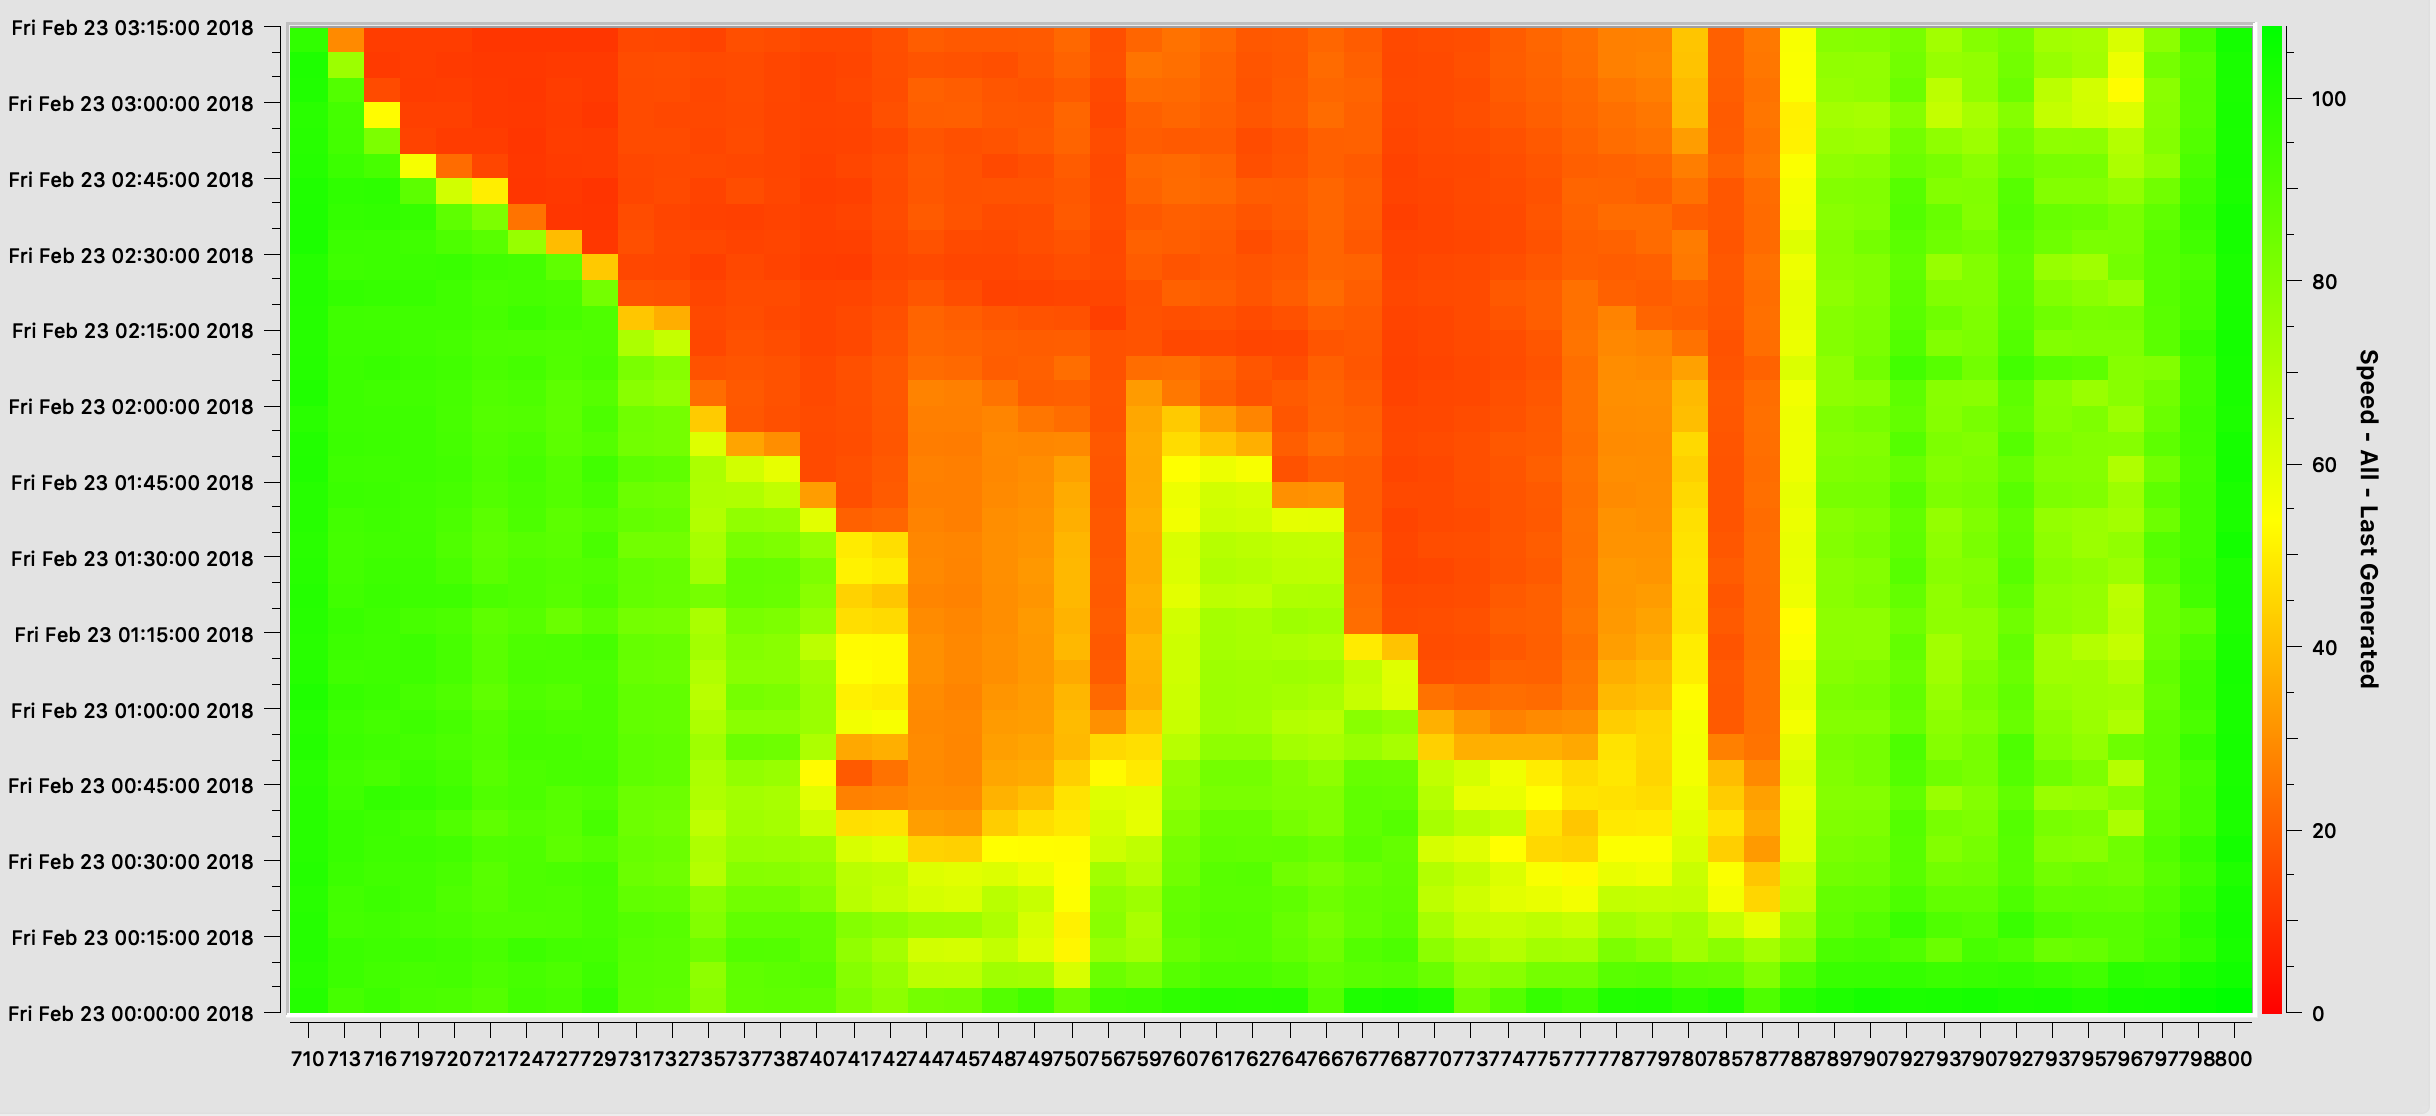
\includegraphics[width=12cm]{increase_20.png}
    \caption{Time-space diagram for simulation with 20\% demand increase}
    \label{fig:increase_20}
\end{figure}

\begin{table}[]
\centering
\caption{Matrics for 20\% Demand Increase}
\begin{tabular}{|l|l|}
\hline
Flow (vph)                    & 8464.31 \\ \hline
Total delay (hr)              & 2322.75 \\ \hline
Average delay (sec/veh)       & 987.90  \\ \hline
Average travel time (sec/veh) & 714.46  \\ \hline
\end{tabular}
\label{20per}
\end{table}

\end{itemize}
As shown in the four simulations above, current operating system of the highway segment could not properly serve an increase in total demand, therefore, new traffic management strategies should be developed to address the issue. Details of development and evaluation of traffic management strategies are described in the next section.


\subsection{Development and Evaluation of Traffic Management Strategies}
In this section, we developed and evaluated three different strategies for improving traffic operations along the test site for the existing and future conditions (20\% increase in traffic demand scenario).


\subsubsection{Ramp Metering}
Ramp Metering is the practice of managing access to a highway via use of control devices such as traffic signals, signing, and gates to regulate the number of vehicles entering or leaving the freeway, which has long been used to limit the number of merges into a recurring bottleneck in order to prevent breakdown of traffic flow. In this section, we applied ramp metering at the selected corridor. Constraints for the practical implementation of the ramp metering strategies were then identified. Finally, we suggested possible mitigation to the constraints.

In our simulations, meter rates are determined according to the capacity and flow at each metered location. The flow rate allowed at each meter is calculated by (capacity of this section - flow from the upstream), according to the lecture [\citeauthor{dkan}, 2019] and examples \cite{askabardonis}. For ramps in uncongested sections, meter rate is arbitrary set at 1-second green in a 2-second cycle. There is actually no need for meters in those sections but, according to the professor, we have to be equitable at all locations. For sections that are moderately congested, meter rates are calculated to range from 400 to 700 vph, which correspond to cycle lengths from ~4s to ~9s. To avoid over-congestion on the ramps, a maximum meter cycle of 10s is set in highly congested areas despite the actual traffic flows, to be equitable. (There is a formula for maximum cycle length, but it is very complicated, and we find 10 to be a good empirical estimation.)

The time-space diagrams for normal and increased demand conditions can be found in Figures \ref{fig:meter} and \ref{fig:meter120}, and metric in Tables \ref{metered} and \ref{metered20}. Figures \ref{fig:meter_ramp} and \ref{fig:meter120ramp} show ramp traffic conditions under normal and increased capacities. From those figures, we can see that, while ramp metering significantly mitigates congestion on the mainline highway, the on-ramps become highly congested. Many highway authorities seem to prioritize the mainline over the ramps, as I often see long lines at on-ramps to I-80 near Berkeley. It is also true that, even without ramp meters, some on-ramps are still very congested as the mainline reaches its full capacity, as Bingyi Fan observed on sections of Massachusetts Turnpike close to inner Boston. How to balance the congestion on the mainline and the ramps deserve further research by the highway authorities.

\begin{figure}
    \centering
    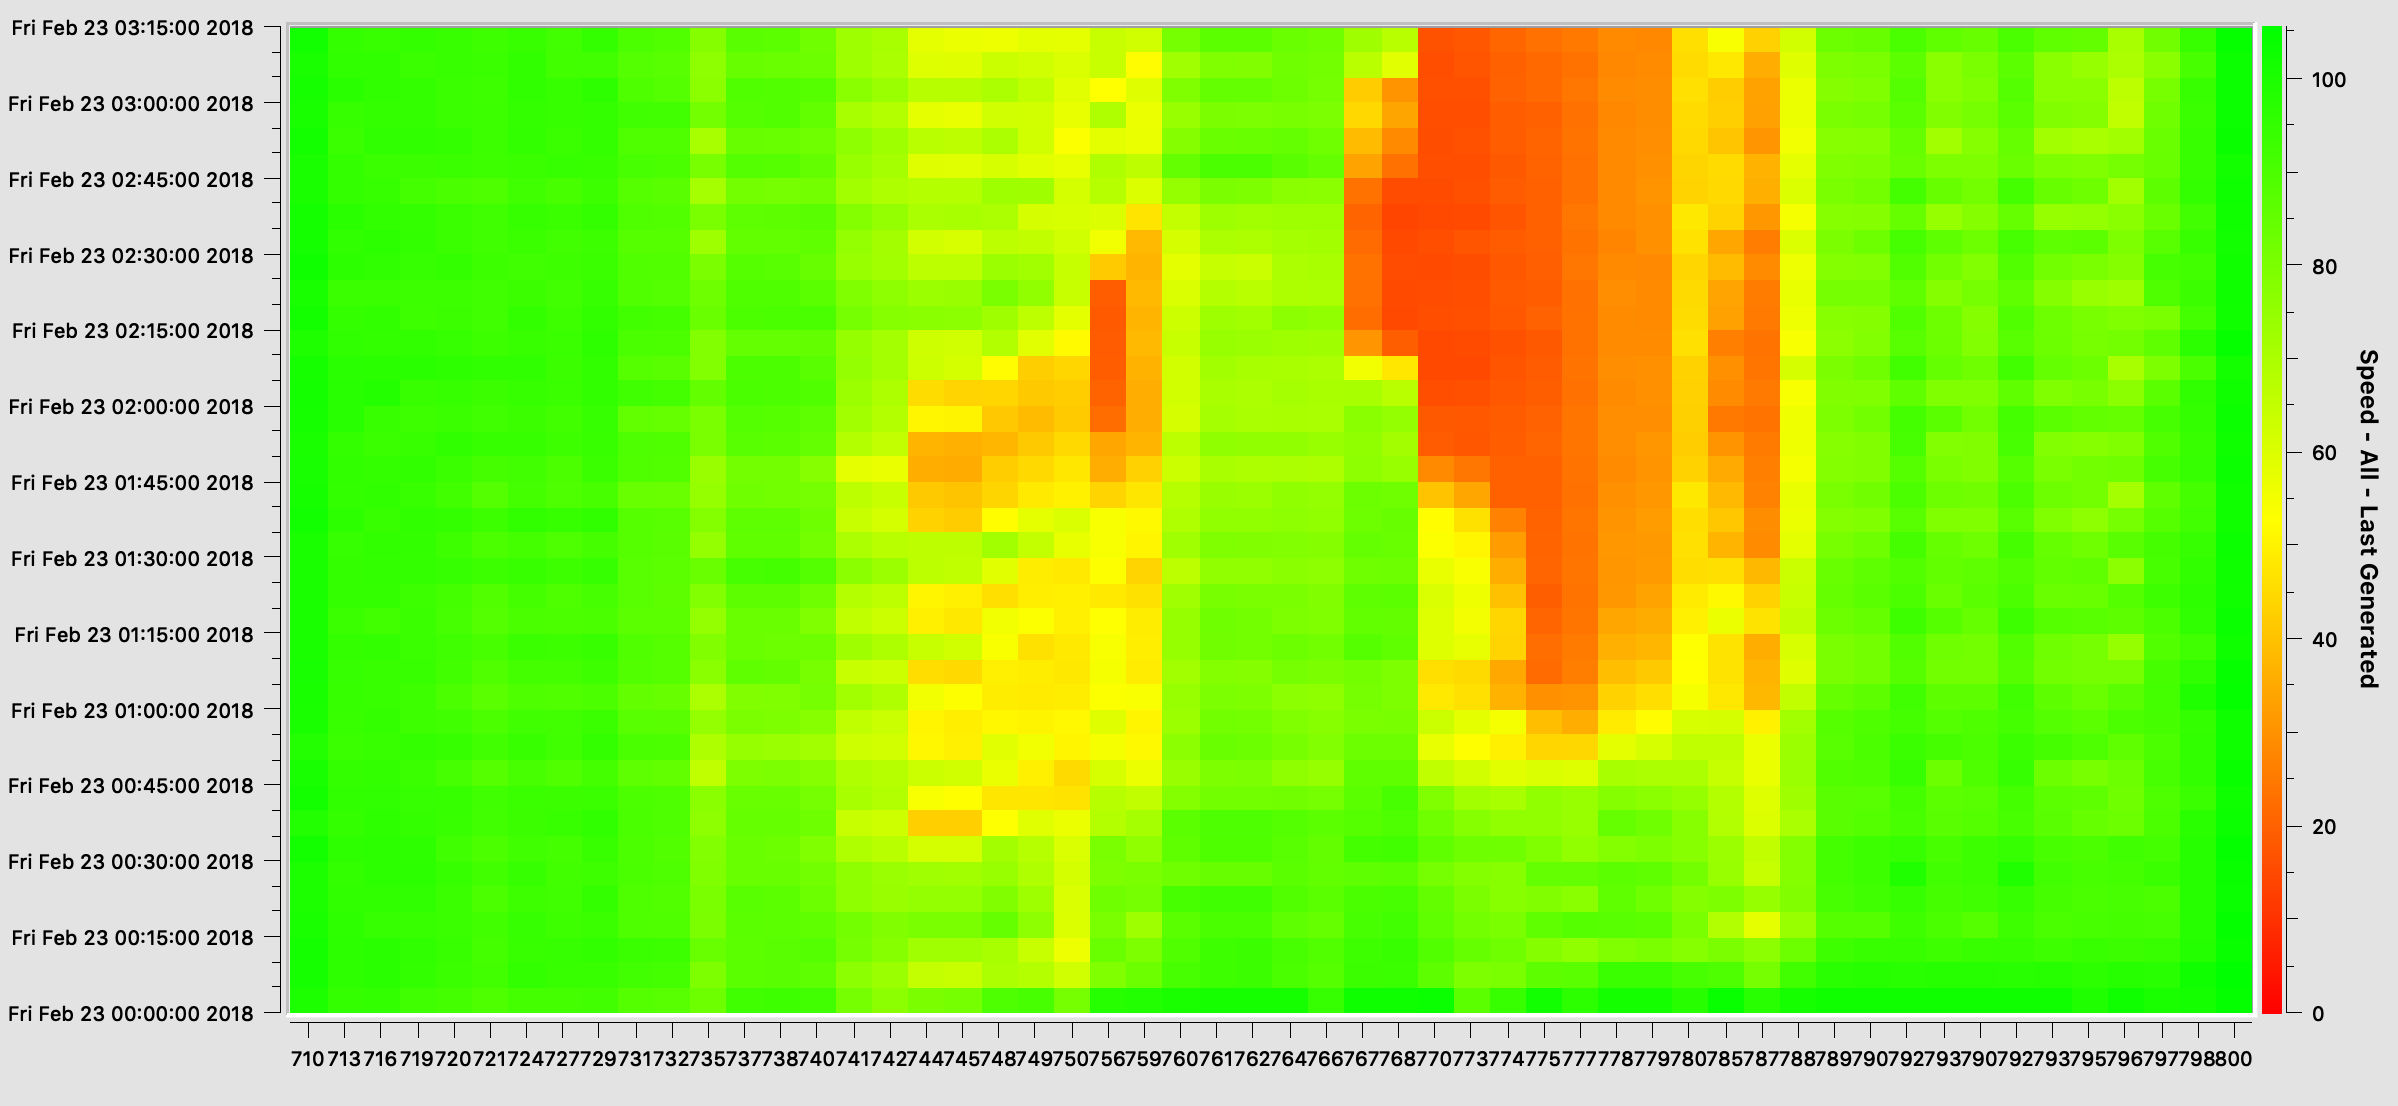
\includegraphics[width=12cm]{metering_normal.png}
    \caption{Time-space diagram for metered highway}
    \label{fig:meter}
\end{figure}
\begin{figure}
    \centering
    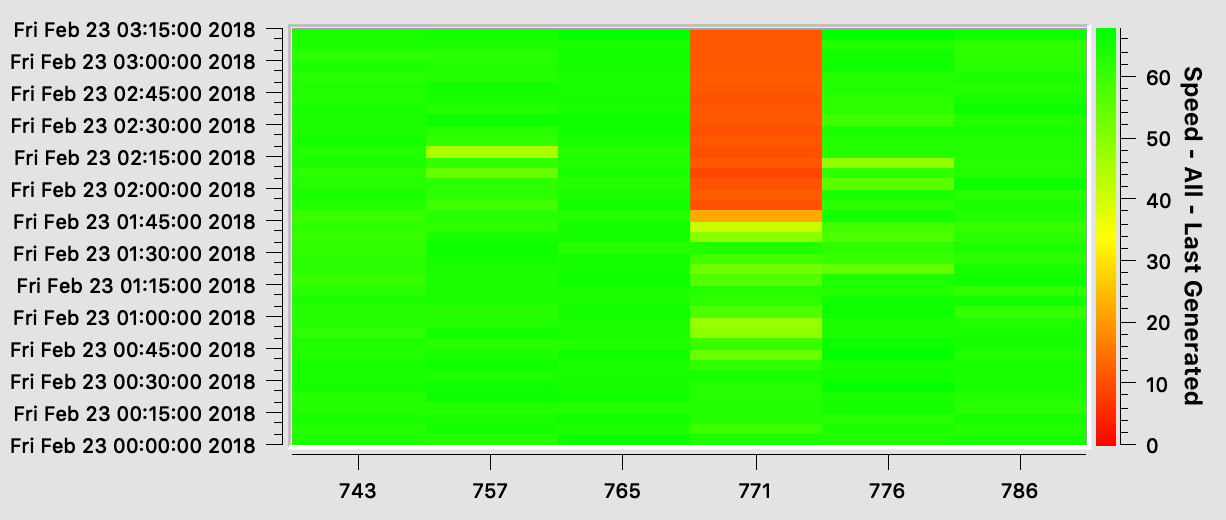
\includegraphics[width=12cm]{metering_normal_ramp.png}
    \caption{Time-space diagram for metered highway ramps}
    \label{fig:meter_ramp}
\end{figure}

\begin{figure}
    \centering
    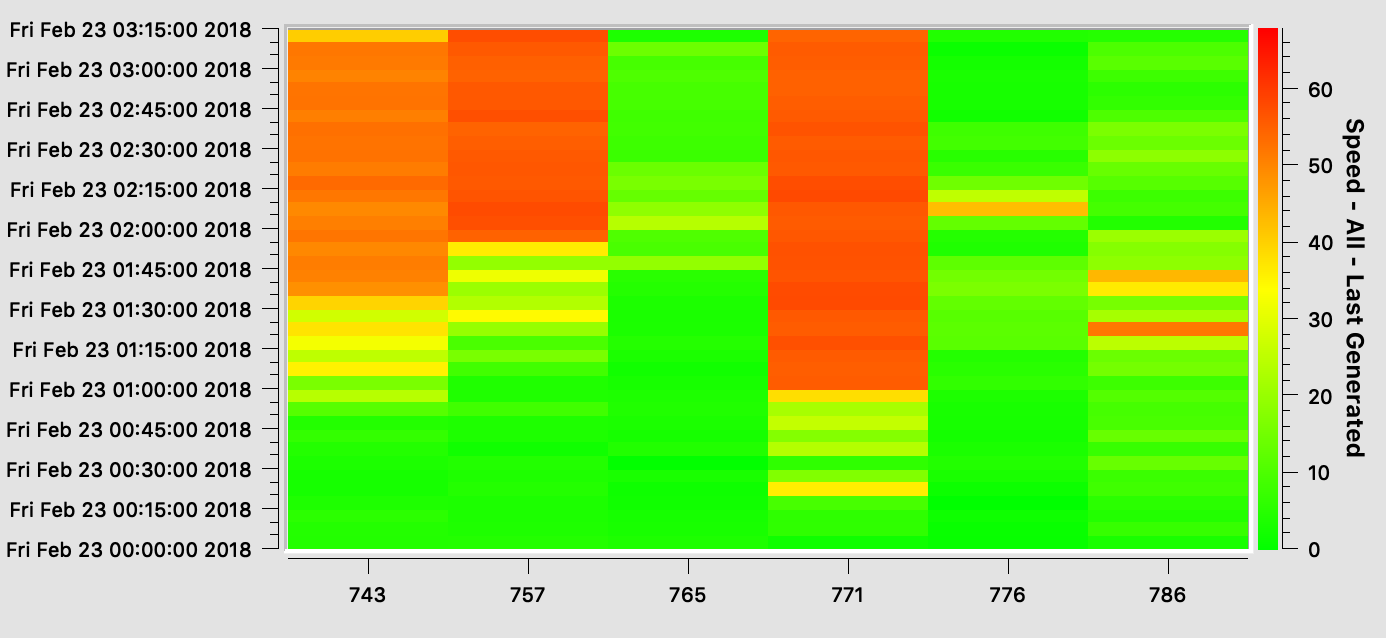
\includegraphics[width=12cm]{metering_120_ramp.png}
    \caption{Time-space diagram for metered highway with 120\% demand}
    \label{fig:meter120}
\end{figure}
\begin{figure}
    \centering
    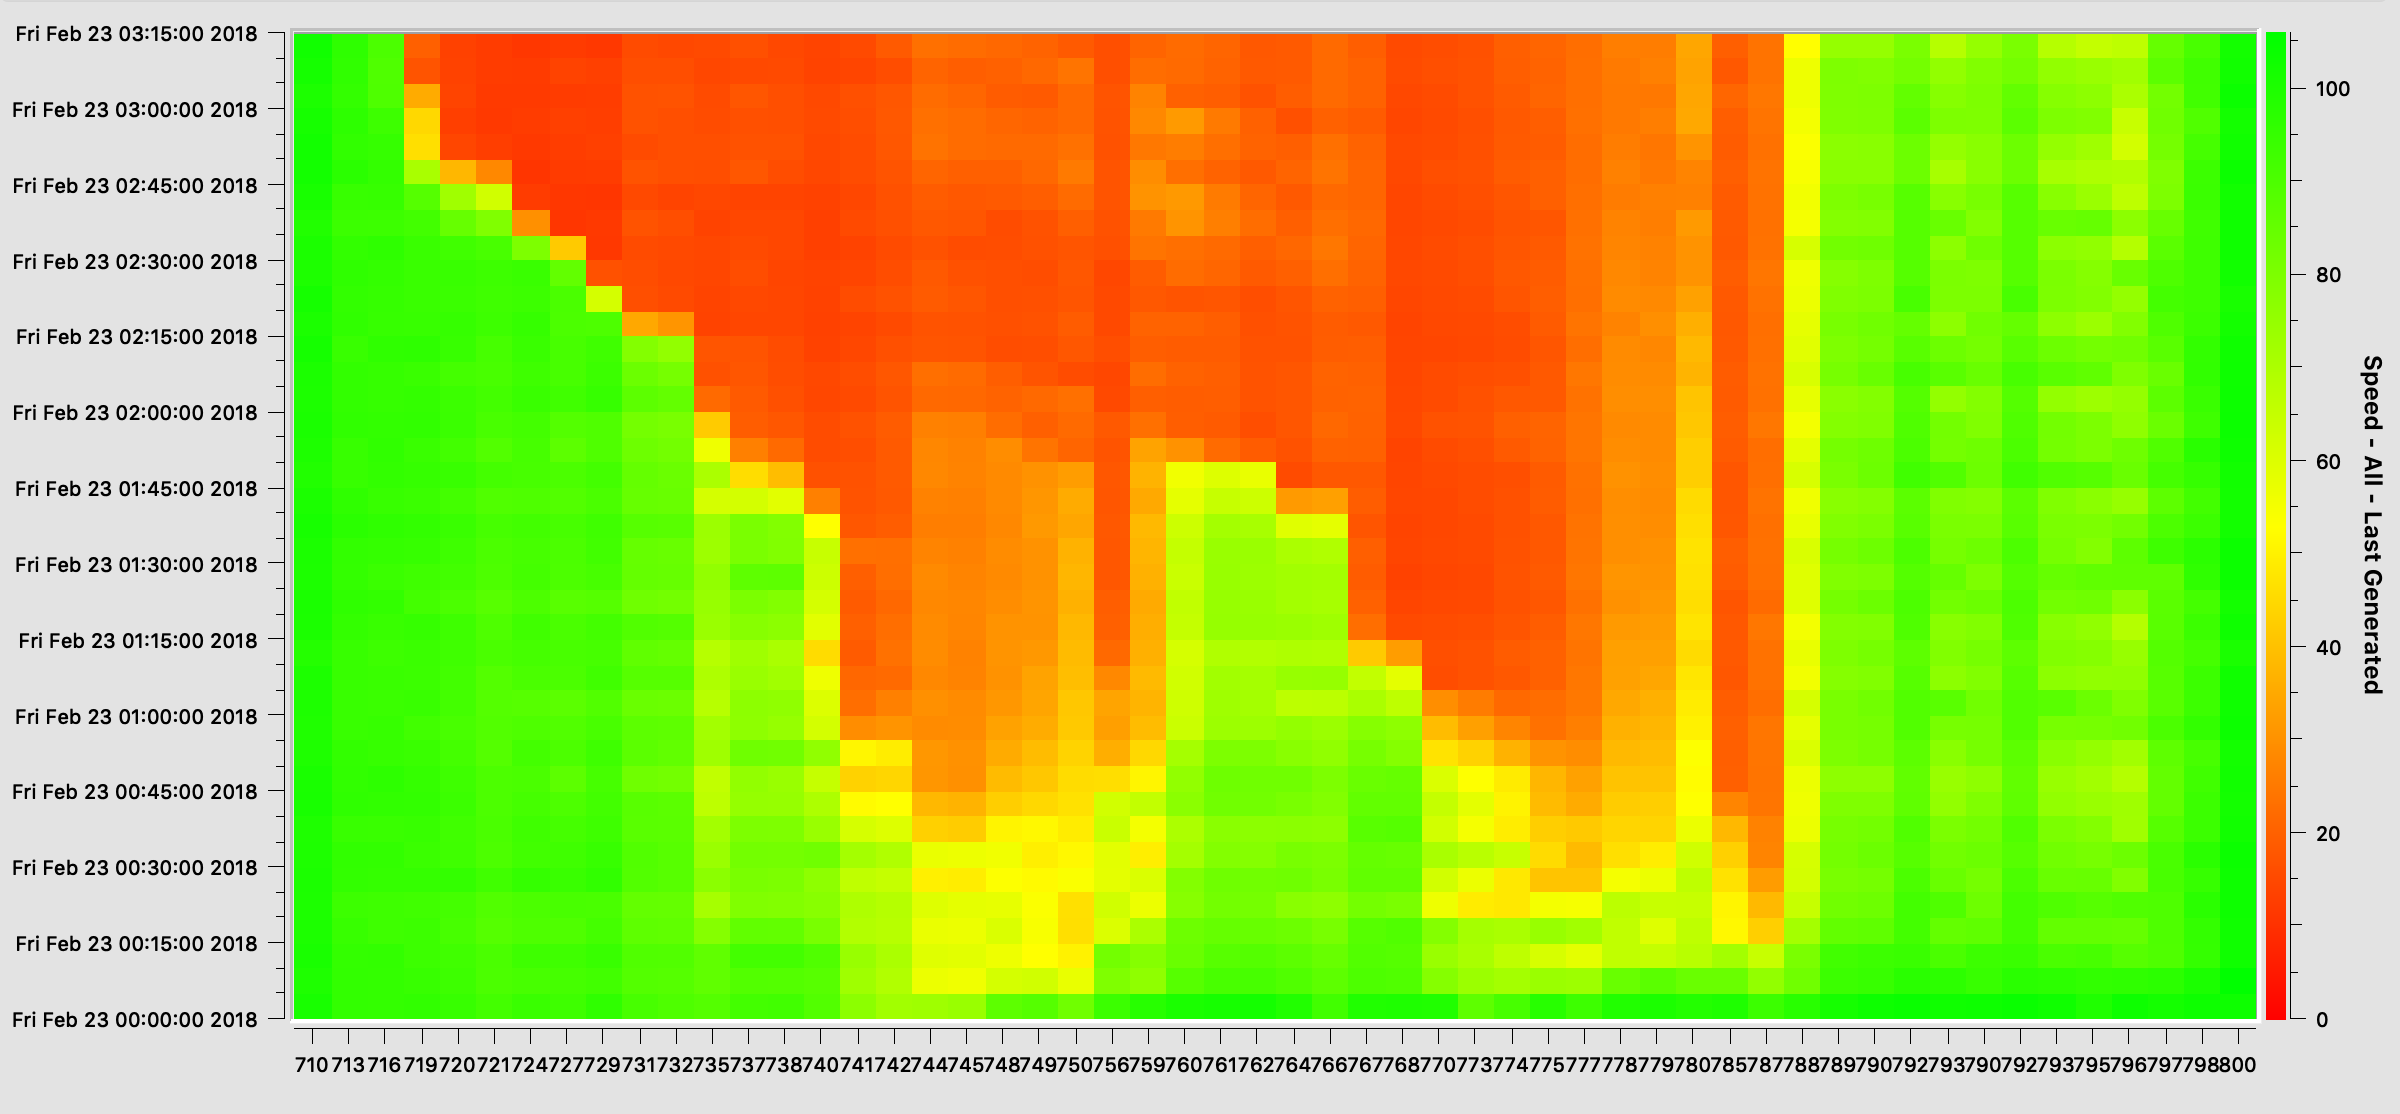
\includegraphics[width=12cm]{metering_120.png}
    \caption{Time-space diagram for metered highway ramps with 120\% demand}
    \label{fig:meter120ramp}
\end{figure}
% We added ramp meters to add on-ramps on the usually congested segments. The meters are set to have a cycle of 7.5 seconds, including a green phase of 2.5 seconds.


\begin{table}[]
\centering
\caption{Metrics of Metered Highway}
\begin{tabular}{|l|l|}
\hline
Flow (vph)                    & 8269.21 \\ \hline
Total delay (hr)              & 834.52  \\ \hline
Average delay (sec/veh)       & 313.69  \\ \hline
Average travel time (sec/veh) & 462.85  \\ \hline
\end{tabular}
\label{metered}
\end{table}

\begin{table}[]
\centering
\caption{Matrics of Metered Highway with 20\% Demand Increase}
\begin{tabular}{|l|l|}
\hline
Flow (vph)                    & 8472.61 \\ \hline
Total delay (hr)              & 2287.85 \\ \hline
Average delay (sec/veh)       & 931.46  \\ \hline
Average travel time (sec/veh) & 692.20  \\ \hline
\end{tabular}
\label{metered20}
\end{table}

In summary, given that ramp metering is beneficial to the whole transportation system only under certain conditions, an auto on-off metering algorithm is recommended. Rather than oscillating on and off, it is suggested that the algorithm starts and ends for AM/PM peak hours based on congestion level.


\subsubsection{Incident Management Measures}
In this section, we evaluated the effectiveness of incident management measures such as faster response and clearance times for lane blocking incidents.

We added periodic section incidents to 7 arbitrarily selected lanes in the usually congested segments. These incidents are set to happen every 30 minutes and last for 5 to 10 minutes each time. We believe that resemble a typical highway incident pattern. Any more frequent incident are unusual.

The time-space diagrams for normal and increased demand conditions can be found in Figures \ref{fig:incident} and \ref{fig:incident20}, and metric in Tables \ref{incident} and \ref{incident20}. We found that, because incidents happen only infrequently and generally cleared up quickly, incidents do not significantly worsen the congestion. In other words, a good incident management plan can certainly improve highway operations, but with limited impacts.

\begin{figure}
    \centering
    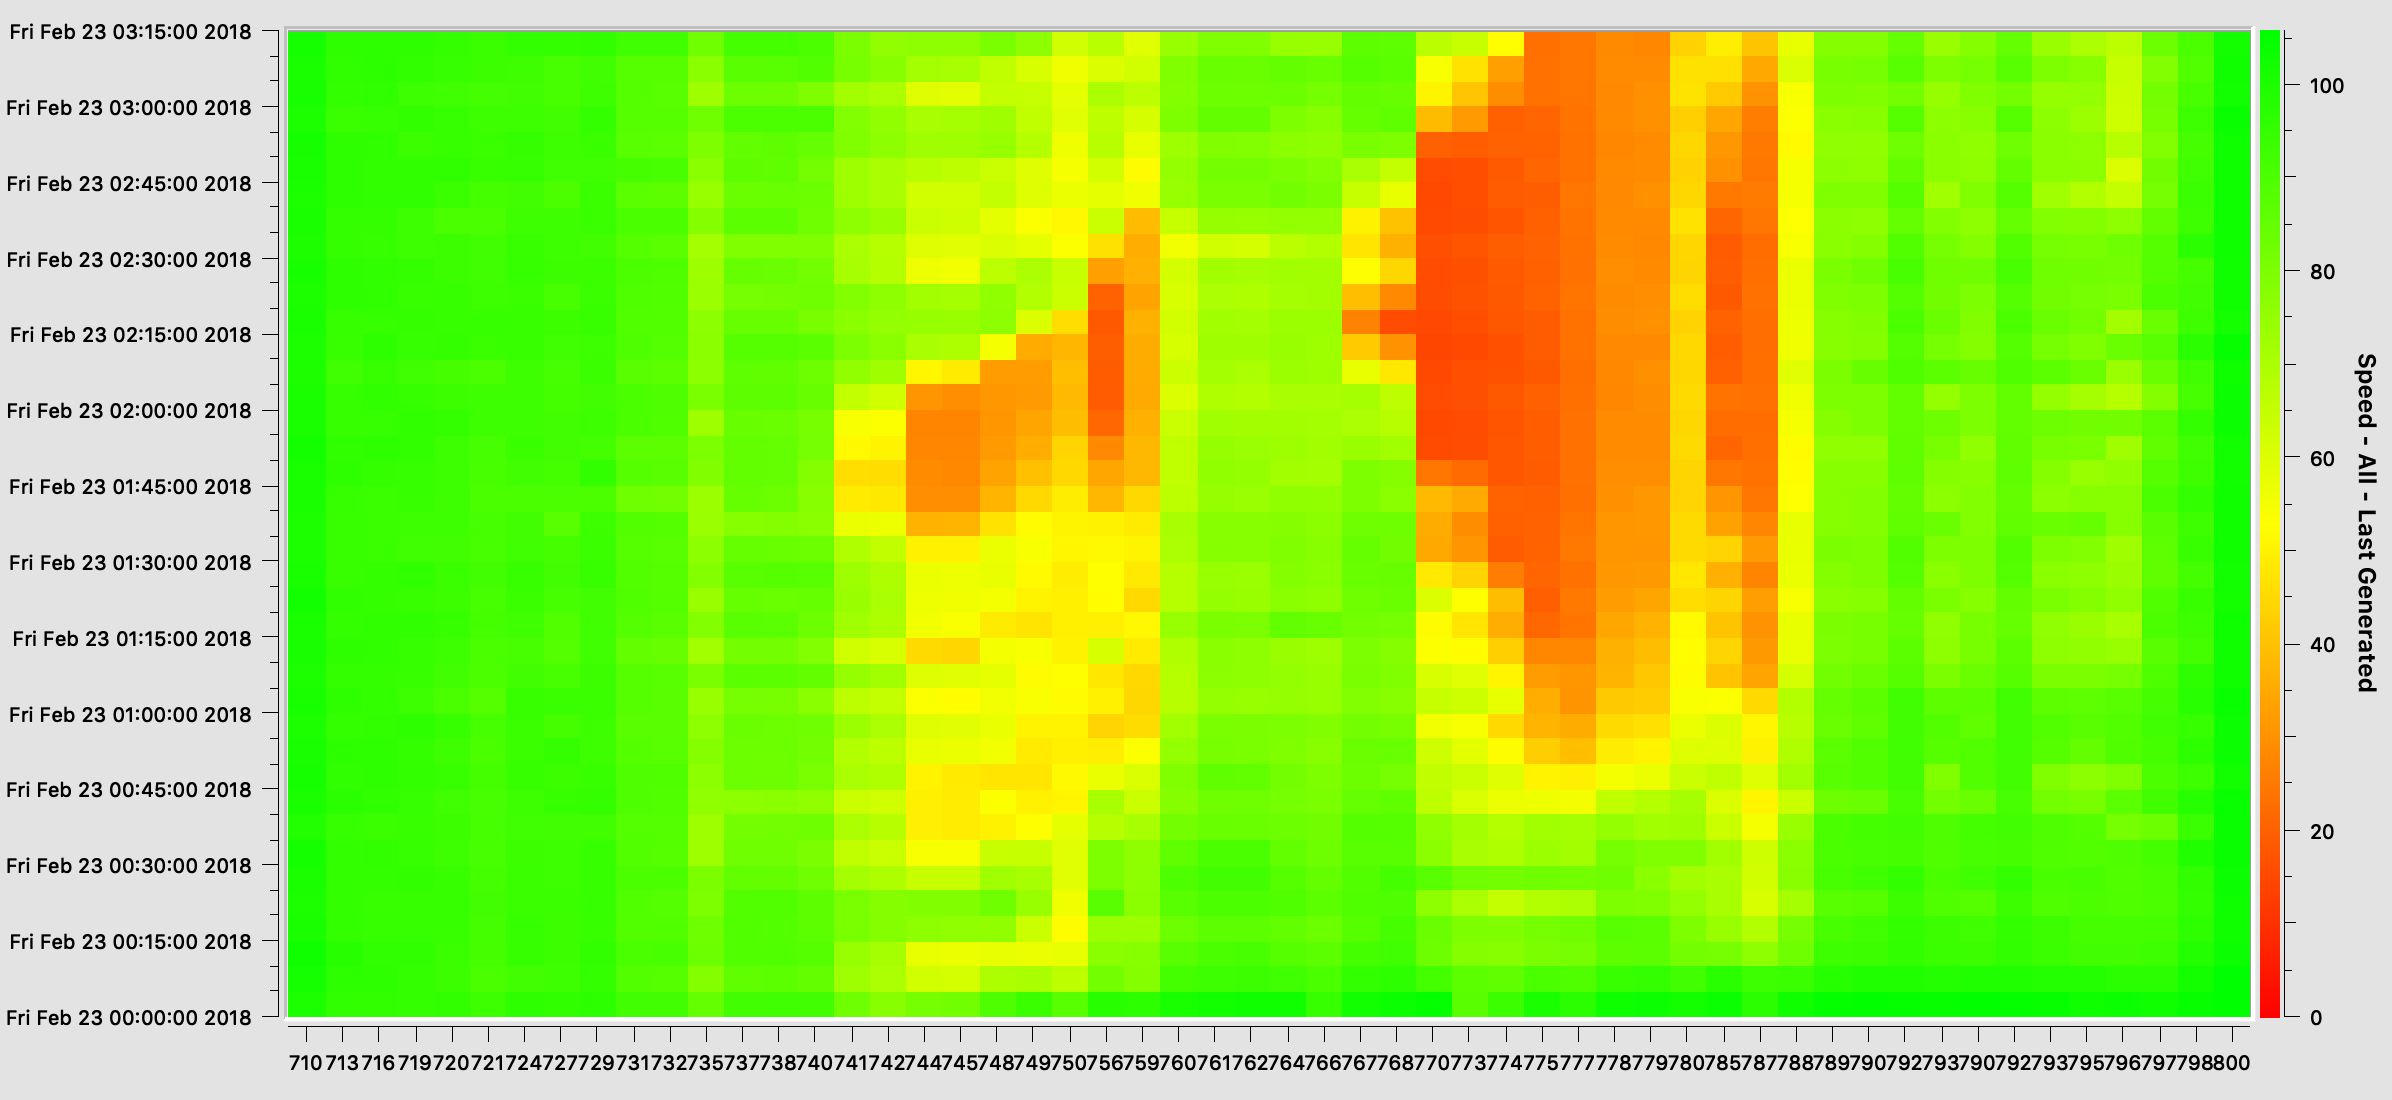
\includegraphics[width=12cm]{incident_normal.png}
    \caption{Time-space diagram for highway with incidents}
    \label{fig:incident}
\end{figure}

\begin{figure}
    \centering
    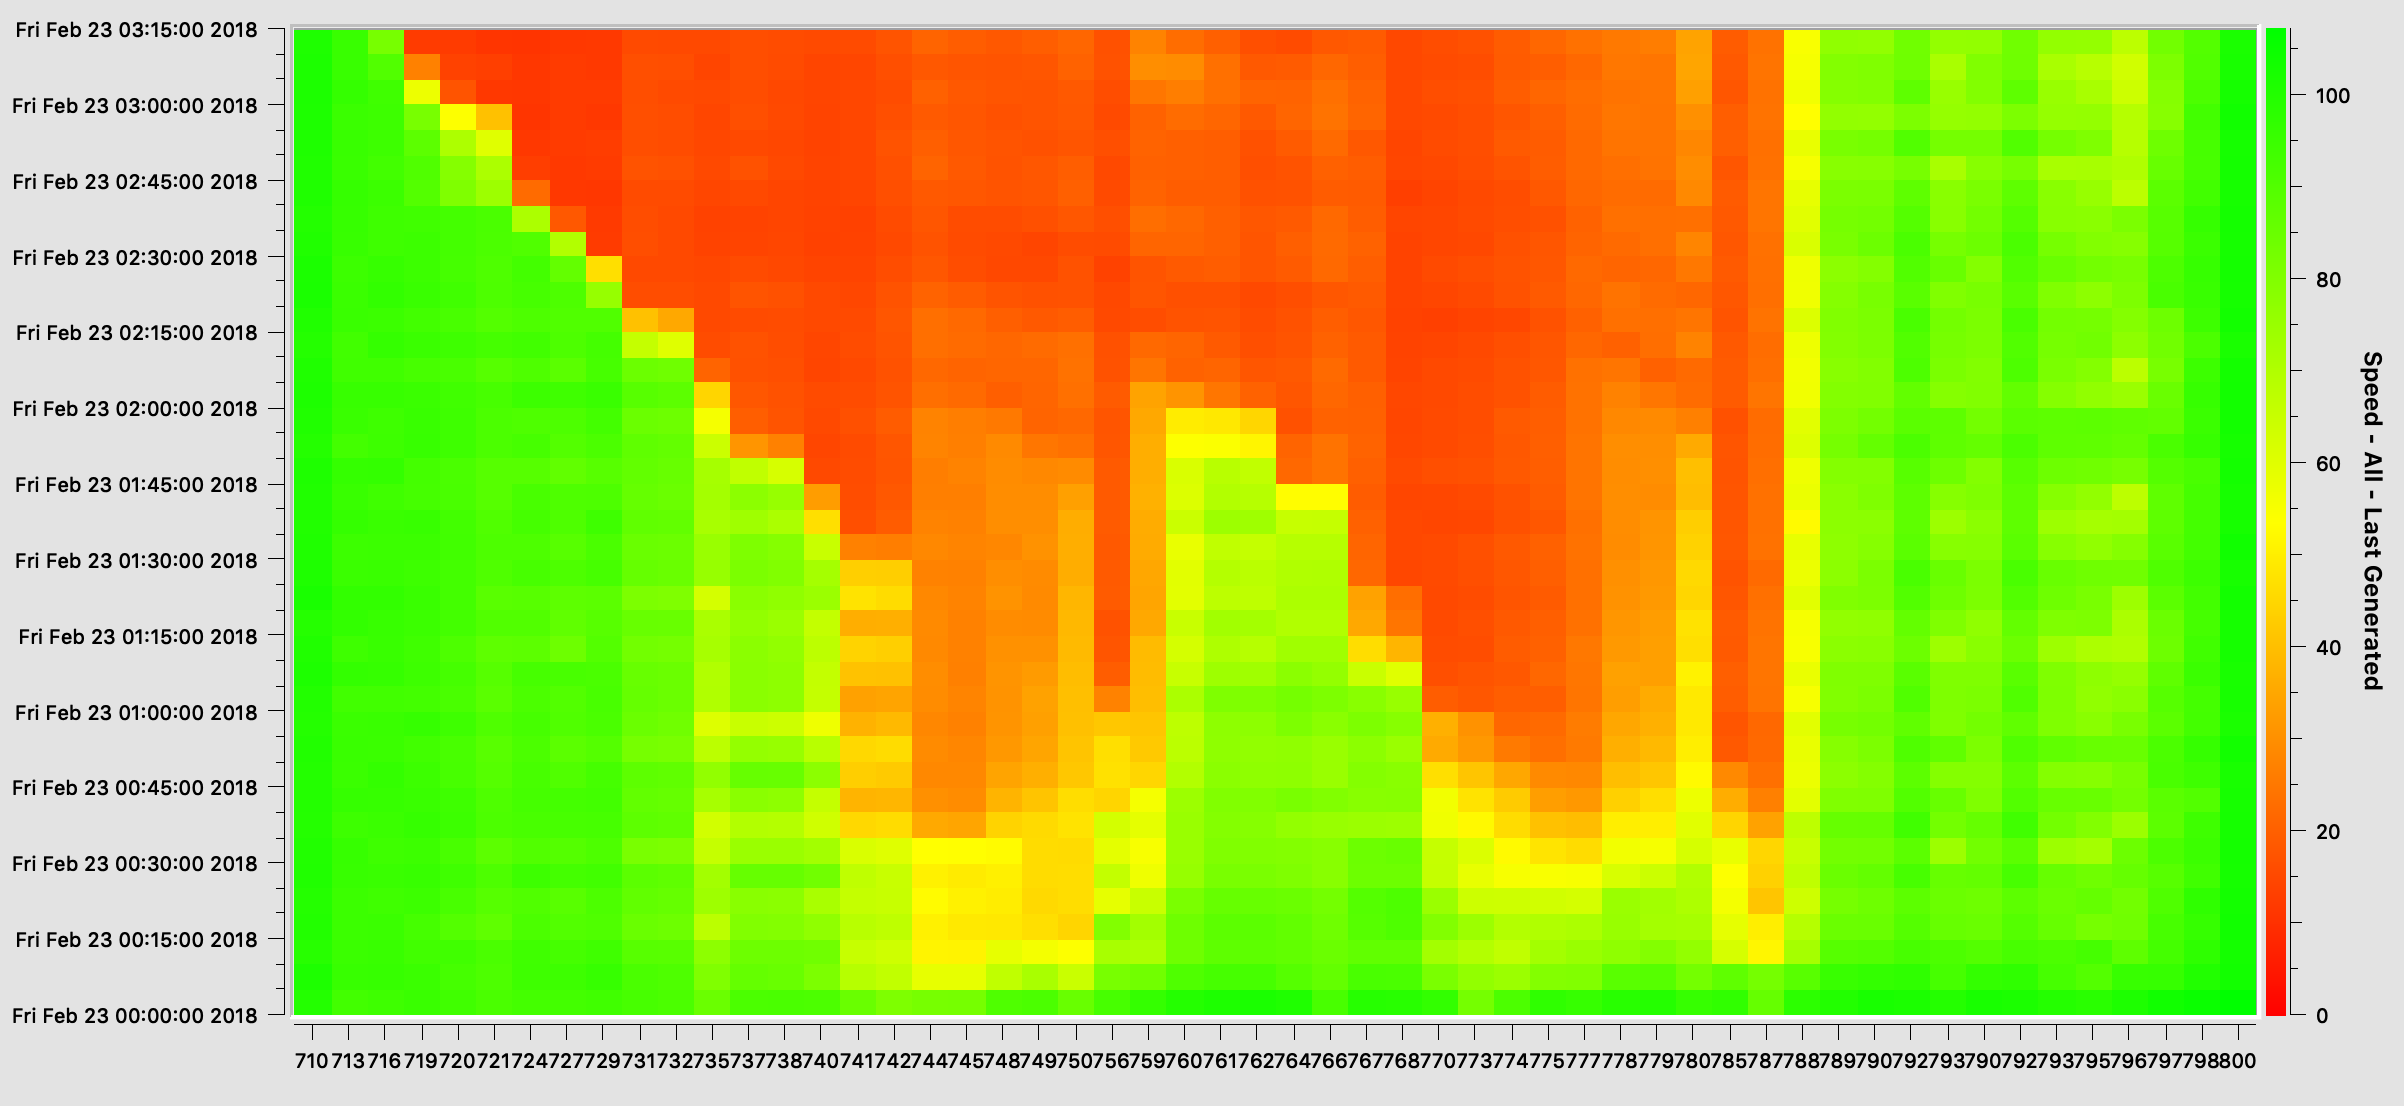
\includegraphics[width=12cm]{incident_120.png}
    \caption{Time-space diagram for highway with incidents and 120\% demand}
    \label{fig:incident20}
\end{figure}

\begin{table}[]
\centering
\caption{Metrics of Highway with Incidents}
\begin{tabular}{|l|l|}
\hline
Flow (vph)                    & 8252.67 \\ \hline
Total delay (hr)              & 841.94  \\ \hline
Average delay (sec/veh)       & 325.09  \\ \hline
Average travel time (sec/veh) & 468.18  \\ \hline
\end{tabular}
\label{incident}
\end{table}

\begin{table}[]
\centering
\caption{Matrics of Highway with Incident and 20\% Demand Increase}
\begin{tabular}{|l|l|}
\hline
Flow (vph)                    & 8469.45 \\ \hline
Total delay (hr)              & 2094.63 \\ \hline
Average delay (sec/veh)       & 952.46  \\ \hline
Average travel time (sec/veh) & 702.25  \\ \hline
\end{tabular}
\label{incident20}
\end{table}

\subsubsection{Geometric and operational improvement}
In this section, we evaluated the effectiveness of geometric and operational improvement at the study freeway section under a proposed expansion. Given that major infrastructure construction projects in the United States are often halted by lack of funding, complexities in land acquisition and lawsuits of all kinds, we proposed a modest expansion plan that require a minimum possible amount of new construction. 

We connected any pair of entry-exit ramps (not exit-entry ones) which is separated by a reasonably short distance. This can be done by expanding the road bed or simply converting the shoulder to a travel lane. This effectively added an additional travel lane on the right side of those segments.

Three such lanes were added in the first congested area and greatly mitigated congestion. Unfortunately, in the second congested area, only 1 such lane could be added due to long distances between the existing ramps. As a result, the mitigation effect of the additional lane on the second congestion is, although significant, limited. Note that the congested ramps in under the increased capacity are caused by the additional demand, not by the expansion. Expansion actually mitigated congestion on the ramps. The ramps are less congested as compared to those under ramp metering, as shown in Figure \ref{fig:meter_ramp}.

An illustration of such an expansion is illustrated in Figure \ref{fig:expand}. The green lane in the upper graph is an entry ramp that ends there, and all vehicles have to merge left. We extended it to the next existing ramp (not shown in graphs), effectively adding a full additional lane in that section. The traffic condition on the rightmost lane, which is currently very congested due to entering and exiting traffic flows, will be greatly mitigated by the addition of lane.

\begin{figure}
    \centering
    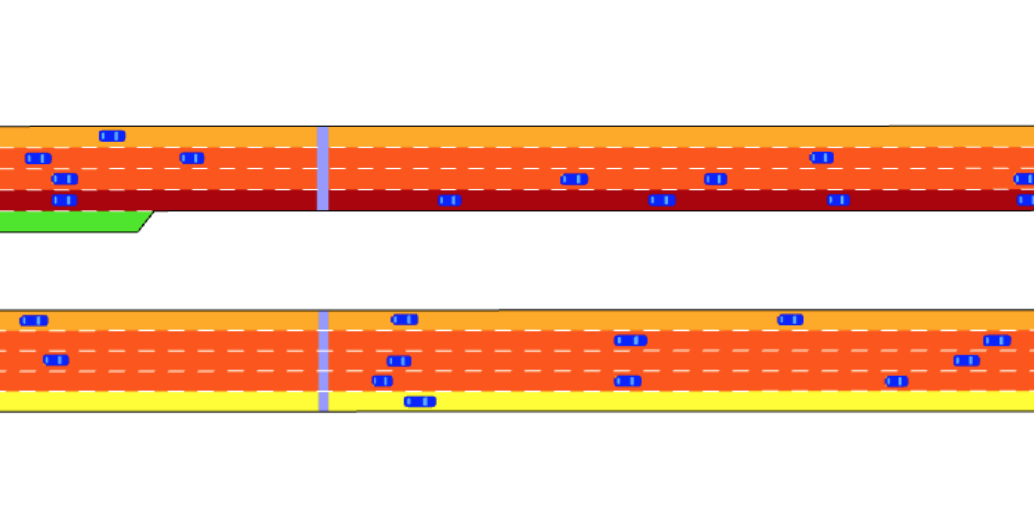
\includegraphics[width=12cm]{add_lane.png}
    \caption{Comparison of Highway Before and After The Proposed Expansion}
    Upper: current condition, with an ended entry ramp and the rightmost lane highly congested. \\
    Lower: condition after a full lane is added in this section. The original rightmost lane is less congested as traffic is re-distributed.
    \label{fig:expand}
\end{figure}

The time-space diagrams for normal and increased demand conditions can be found in Figures \ref{fig:expansion} and \ref{fig:expansion120}, and metric in Tables \ref{expansion} and \ref{expansion120}. Figures \ref{fig:expansion_ramp} and \ref{fig:expansion_ramp120} show ramp traffic conditions under normal and increased capacities. We can see that a physical expansion of the highway not only reduces congestion on the mainline, but also avoid adding congestion to the ramps, as would metering do.

\begin{figure}
    \centering
    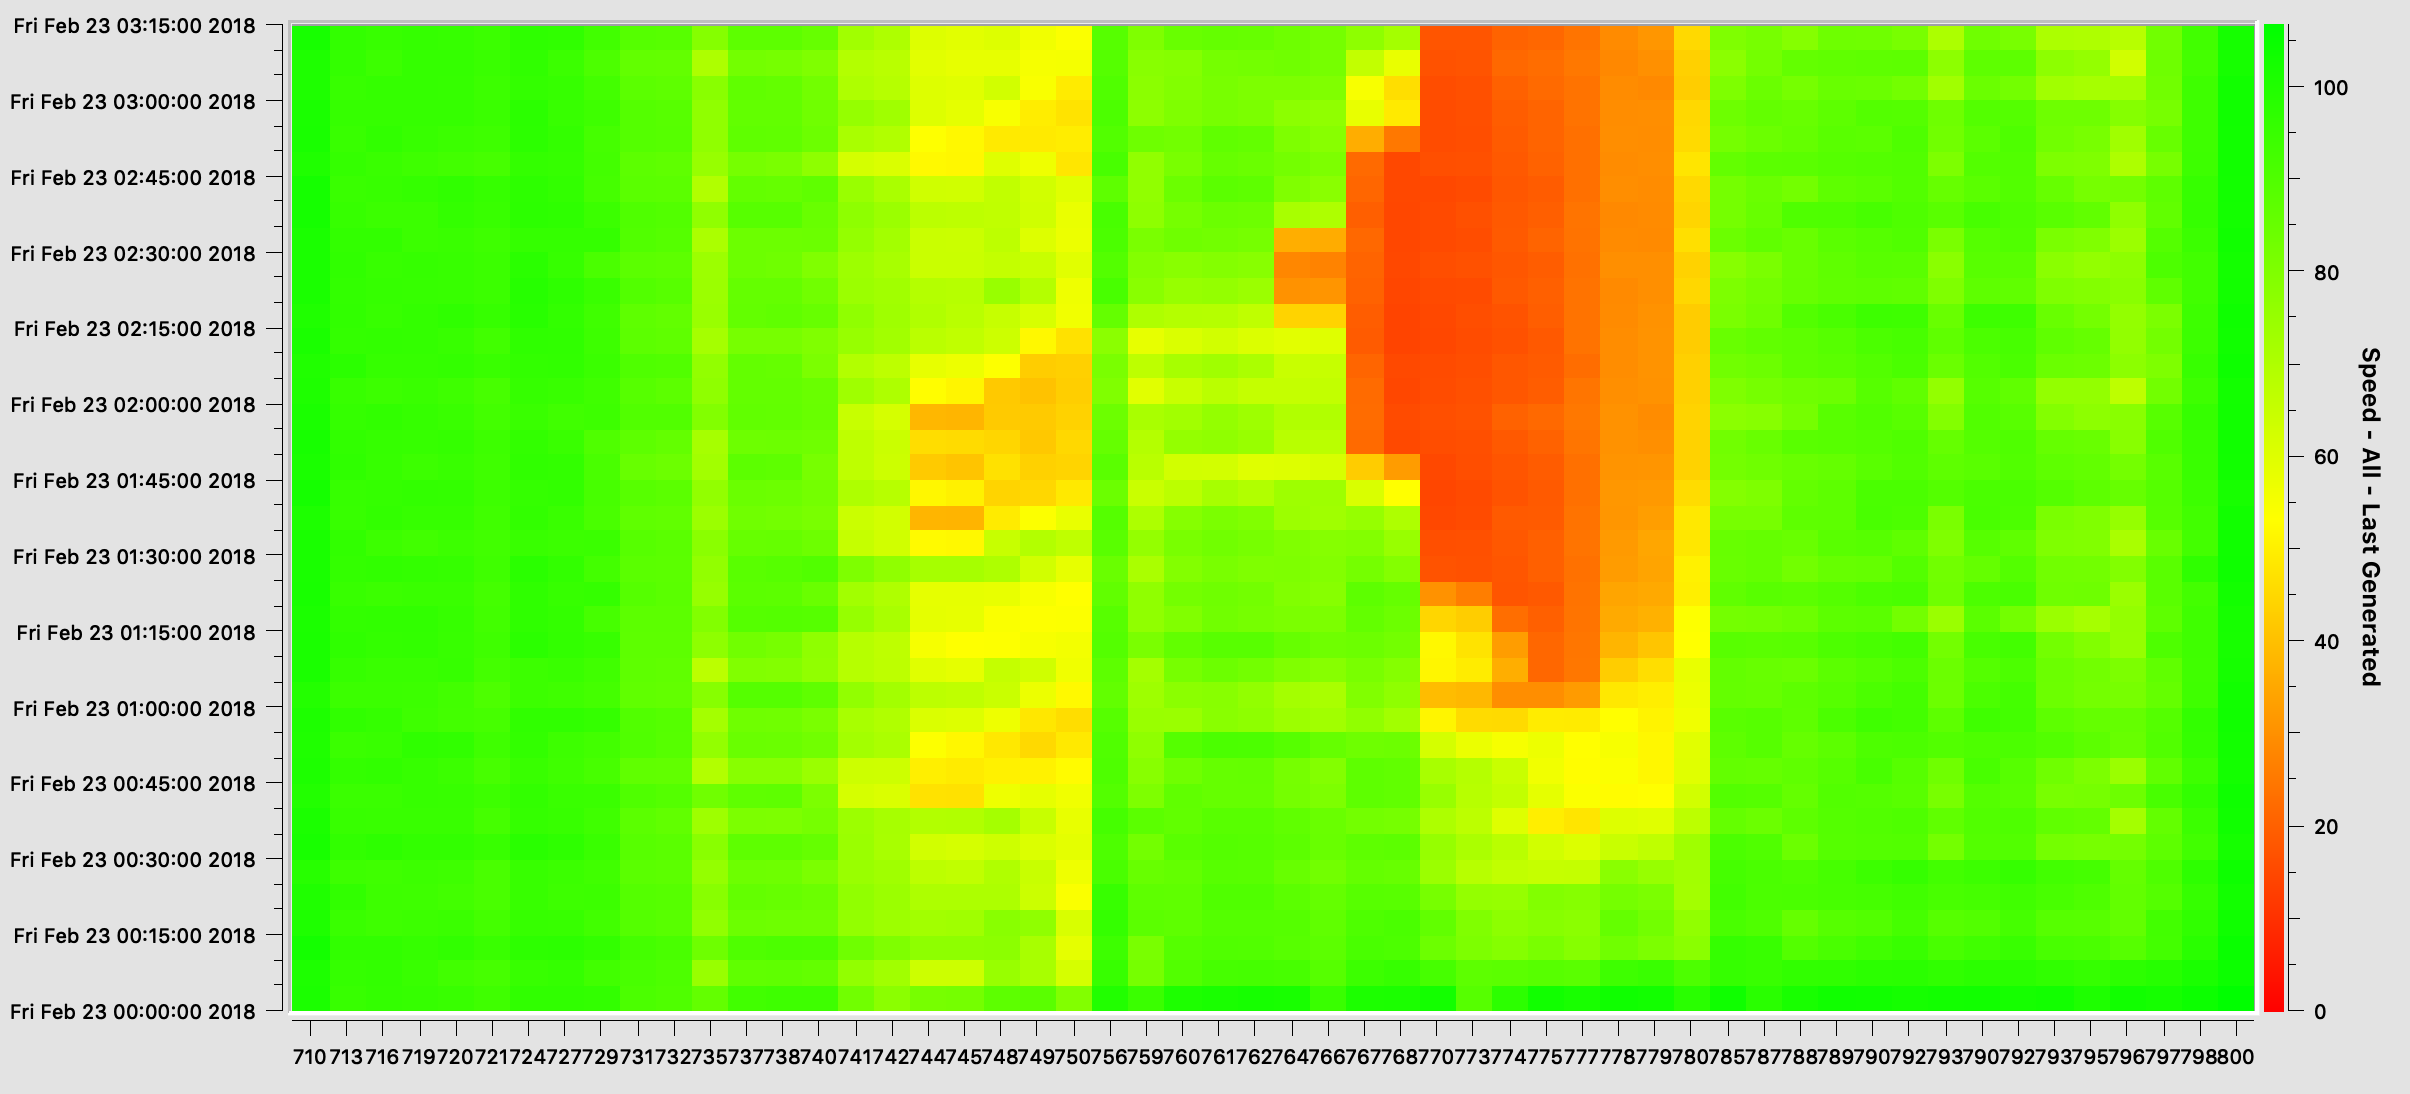
\includegraphics[width=12cm]{addlane_normal.png}
    \caption{Time-space diagram for expanded highway}
    \label{fig:expansion}
\end{figure}

\begin{figure}
    \centering
    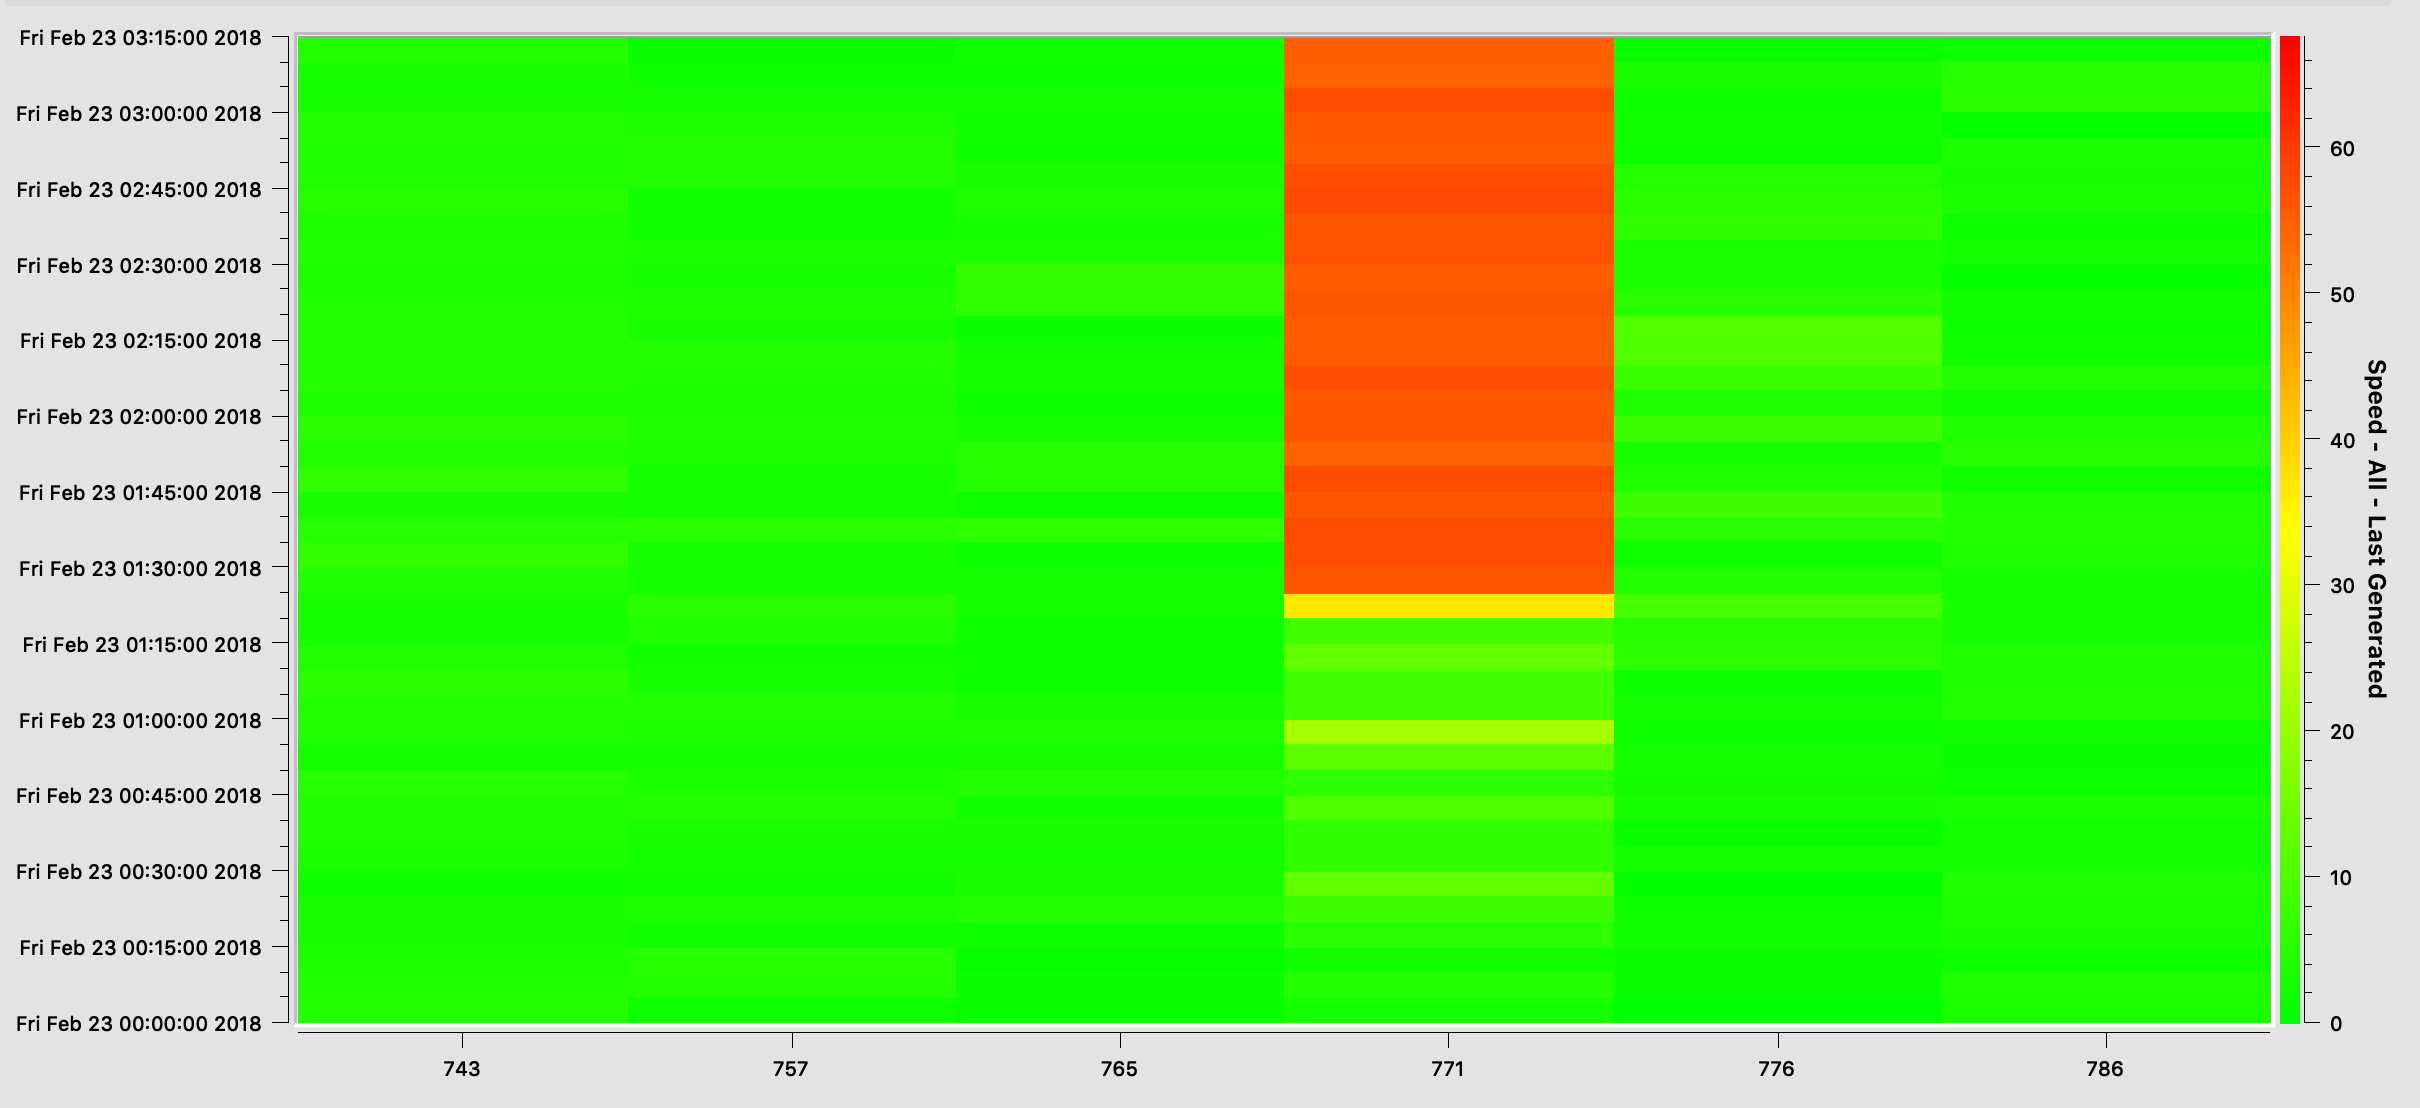
\includegraphics[width=12cm]{addlane_normal_ramp.png}
    \caption{Time-space diagram for ramps on the expanded highway}
    \label{fig:expansion_ramp}
\end{figure}

\begin{figure}
    \centering
    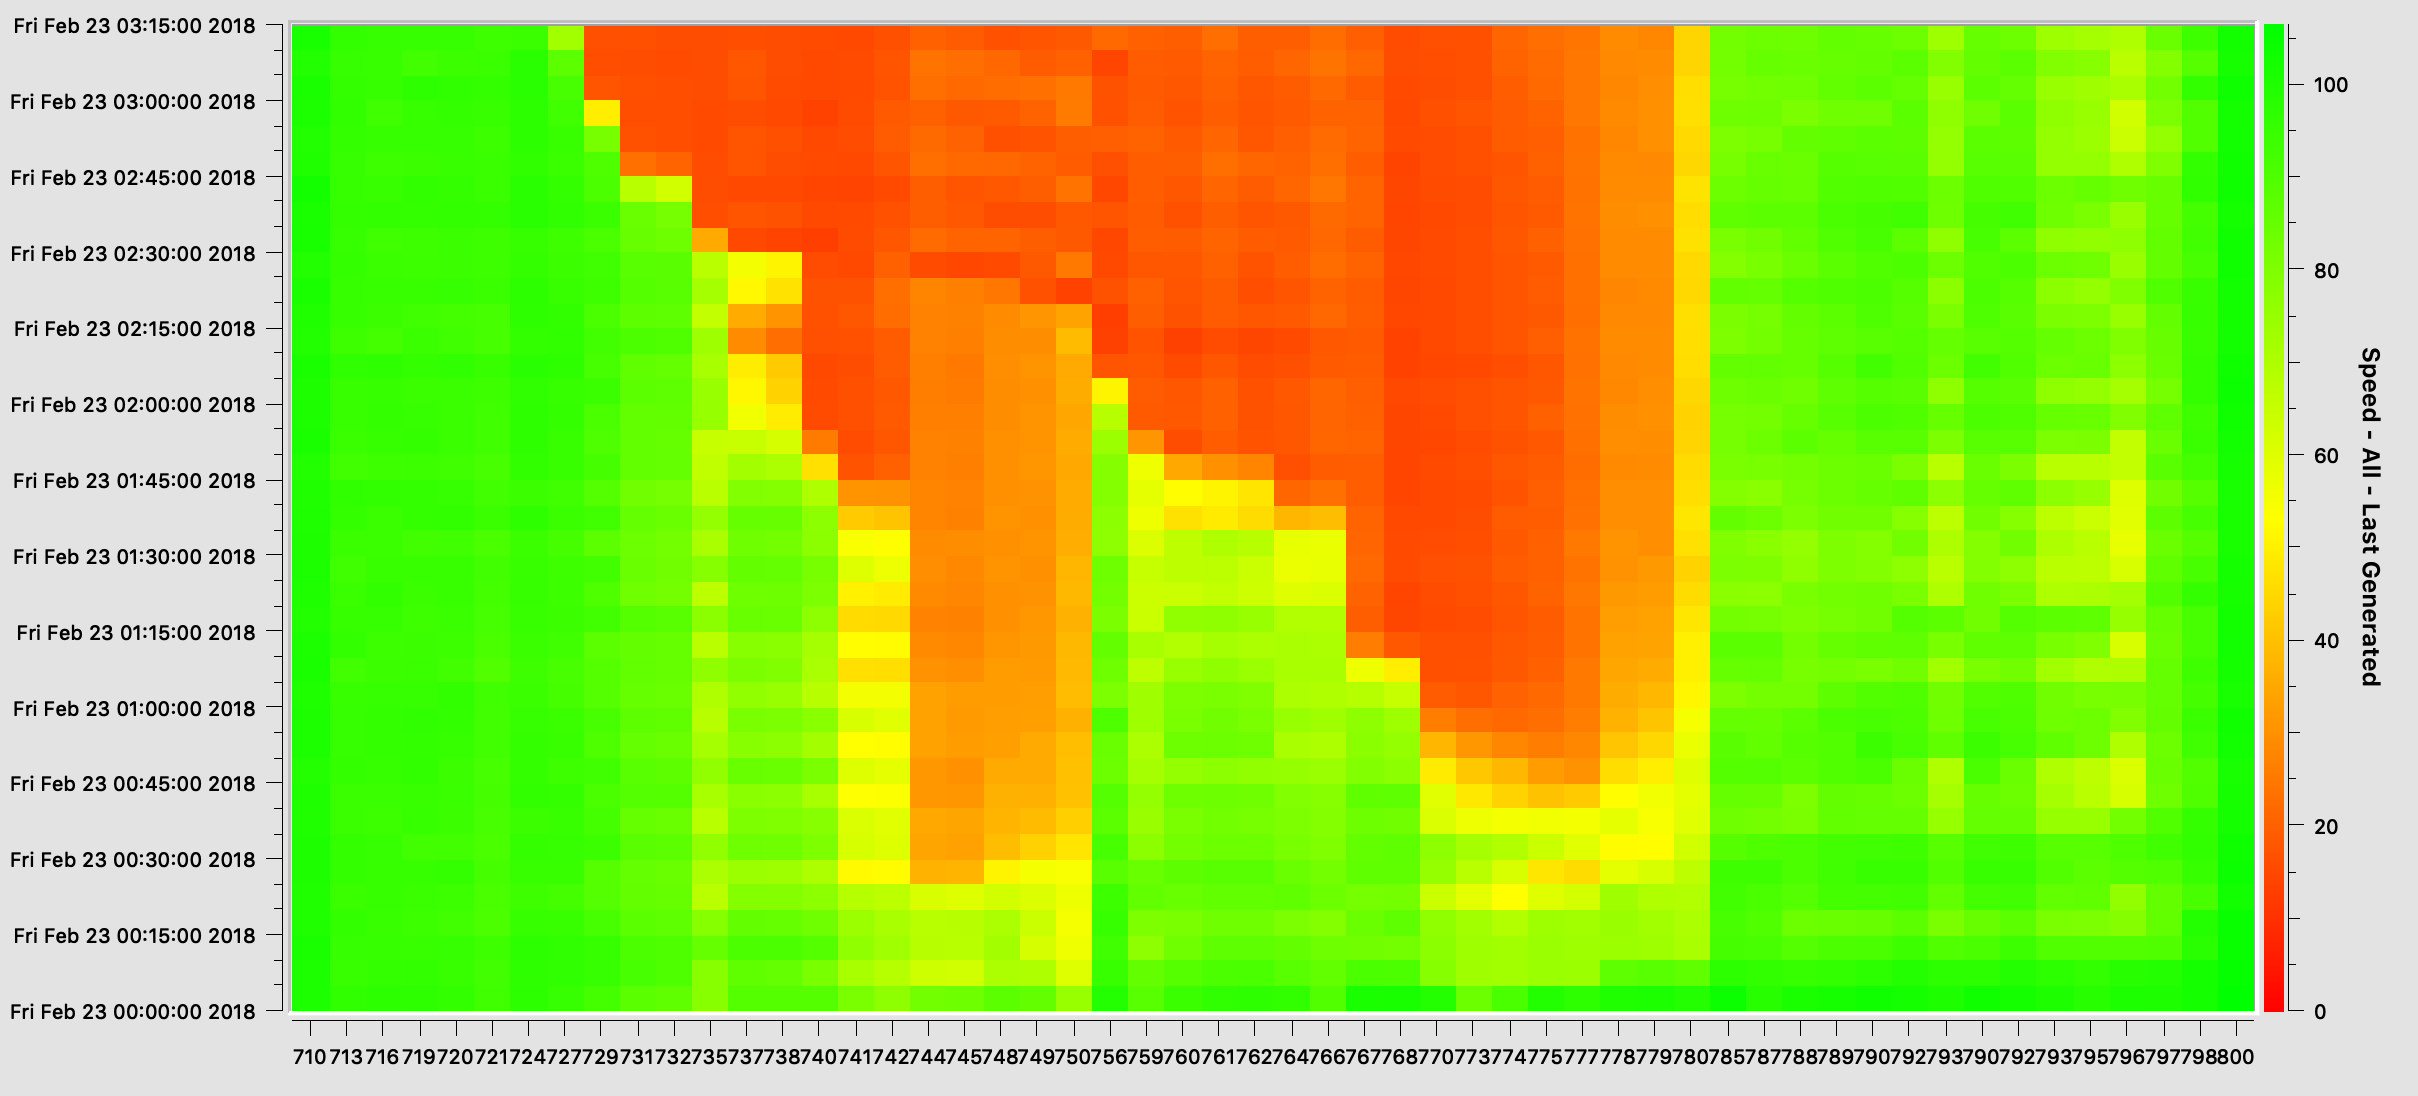
\includegraphics[width=12cm]{addlane_120.png}
    \caption{Time-space diagram for expanded highway with 120\% demand}
    \label{fig:expansion120}
\end{figure}

\begin{figure}
    \centering
    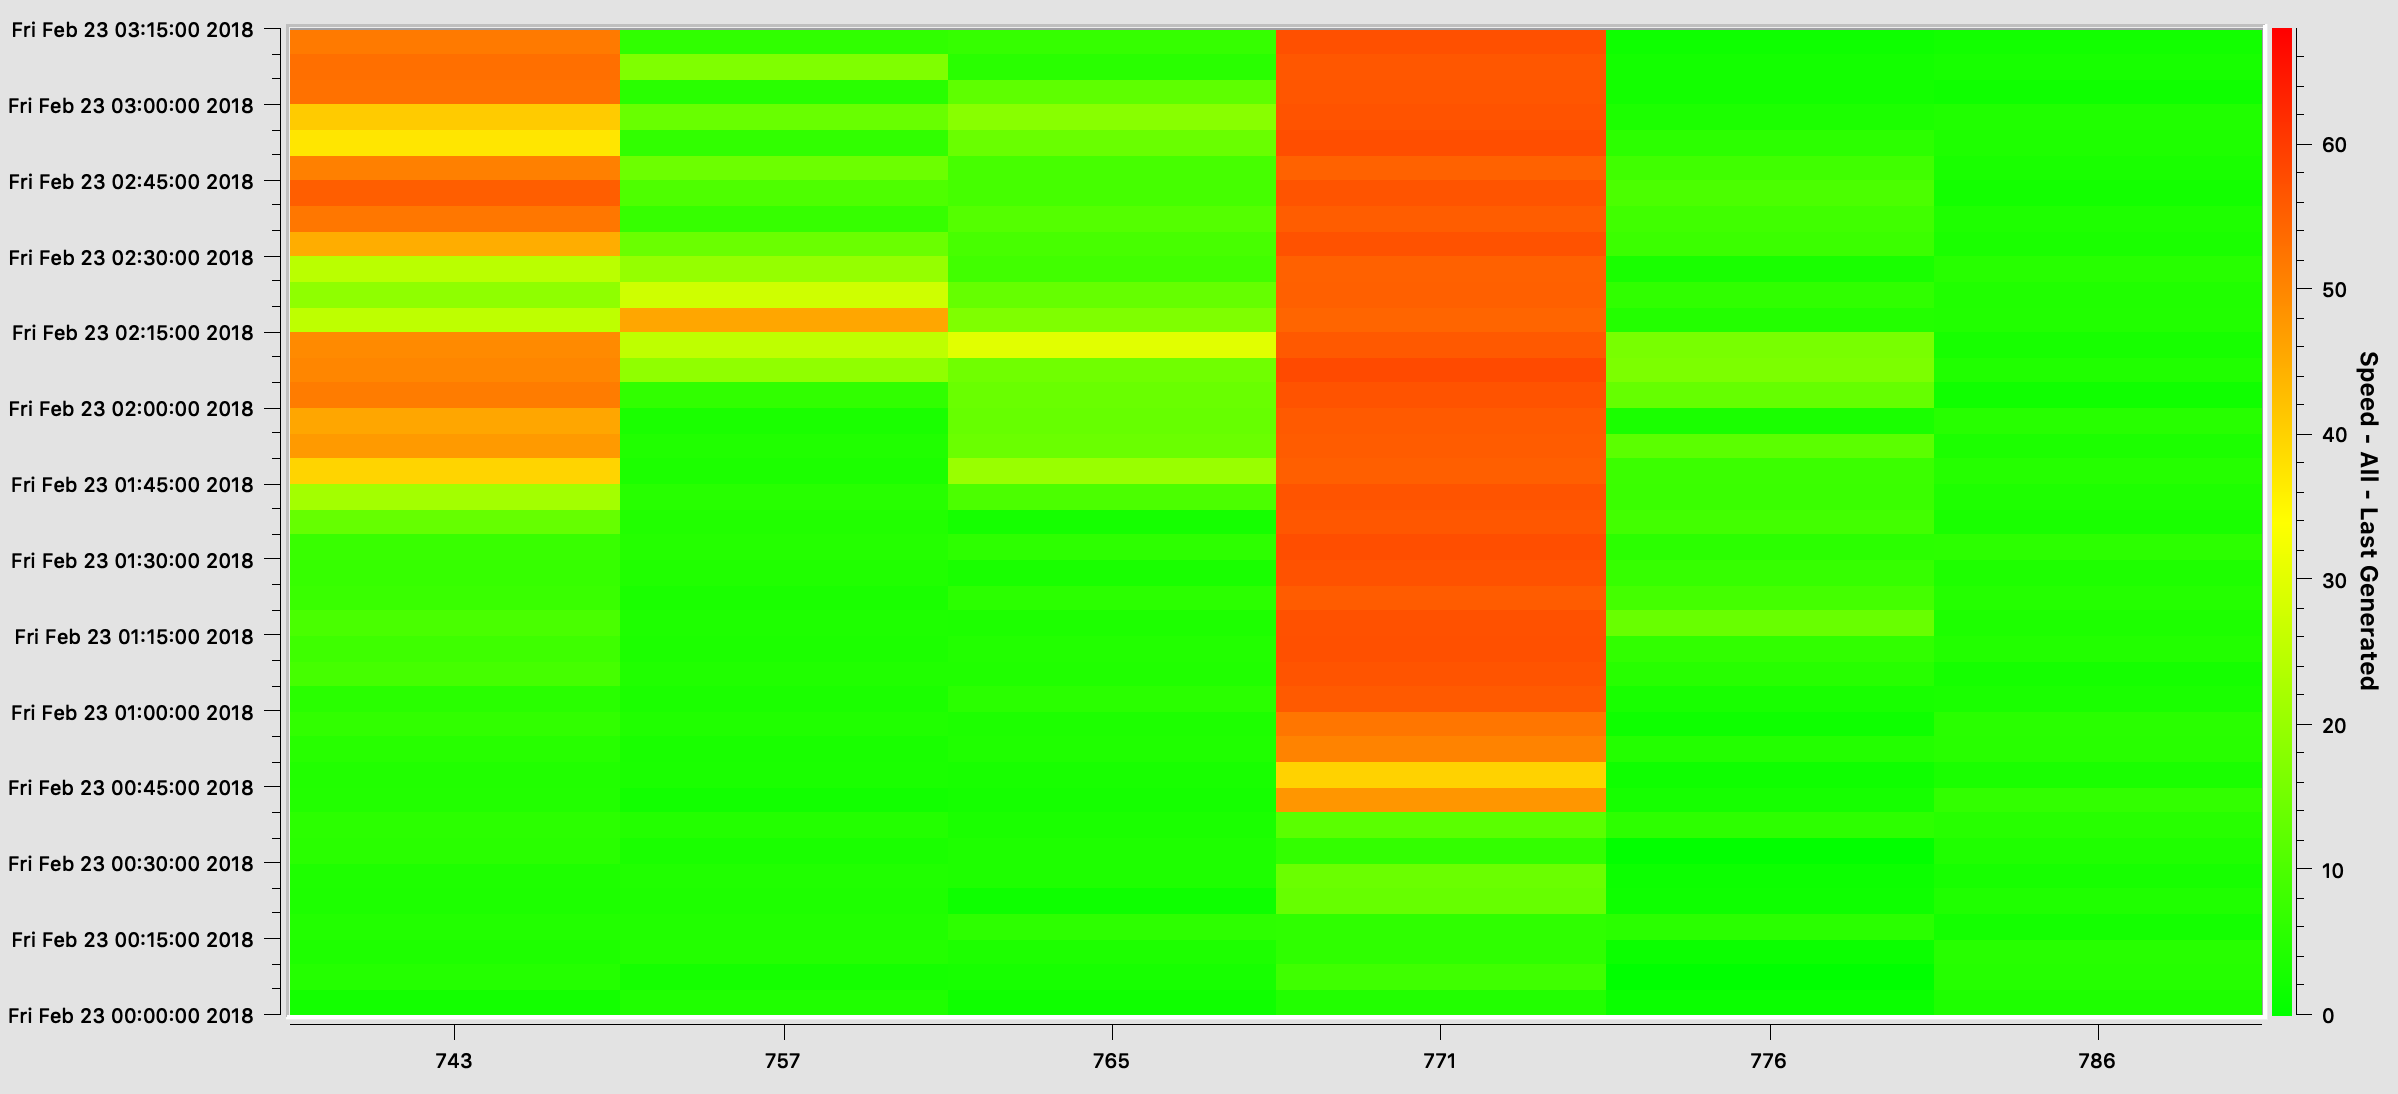
\includegraphics[width=12cm]{addlane_120_ramp.png}
    \caption{Time-space diagram for ramps on the expanded highway with 120\% demand}
    \label{fig:expansion_ramp120}
\end{figure}

\begin{table}[]
\centering
\caption{Metrics of Expanded Highway}
\begin{tabular}{|l|l|}
\hline
Flow (vph)                    & 8259.32 \\ \hline
Total delay (hr)              & 836.86  \\ \hline
Average delay (sec/veh)       & 277.59  \\ \hline
Average travel time (sec/veh) & 324.47  \\ \hline
\end{tabular}
\label{expansion}
\end{table}

\begin{table}[]
\centering
\caption{Matrics of Expanded Highway with 20\% Demand Increase}
\begin{tabular}{|l|l|}
\hline
Flow (vph)                    & 8470.36 \\ \hline
Total delay (hr)              & 2304.63 \\ \hline
Average delay (sec/veh)       & 952.46  \\ \hline
Average travel time (sec/veh) & 702.25  \\ \hline
\end{tabular}
\label{expansion120}
\end{table}


% %%%%%%%%%%%%%%%%%%%%%%%%%%%%%%%%%%%%%%%
% % Results 
% %%%%%%%%%%%%%%%%%%%%%%%%%%%%%%%%%%%%%%%
% \section{Results}
% Analyze the simulation results and document the changes in traffic performance for the entire network, mainline and ramps. Recommend the most promising strategies for the study section.


%%%%%%%%%%%%%%%%%%%%%%%%%%%%%%%%%%%%%%%
% Conclusions 
%%%%%%%%%%%%%%%%%%%%%%%%%%%%%%%%%%%%%%%
\section{Conclusions}
In summary, the group determined that both of limited ramp metering and lane addition to the highway would substantially mitigate congestion on the highway. Lane addition is the best option, provided sufficient funding, because it avoids congesting the ramps. However, it should also be taken into consideration that, during the construction period, traffic conditions will most likely be worsened. A good incident management plan can improve highway operational performance but with limited impacts. With the high cost of lane addition, it is most practical to apply ramp metering in real-world scenarios. Our findings are validated by the fact that ramp-metering is the most popular highway traffic management approach in the U.S. nowadays. %其实很多地方就是让他堵着hhhhh
To improve the effects of ramp metering, it is also possible to use real-time meter control instead of pre-timed meters. The meter rate can be determined by a centralized controller on the real-time data of traffic flows.


\newpage
\bibliographystyle{plainnat}
\bibliography{references}
% Reference:
% http://www.dot.ca.gov/trafficops/tech/docs/RMDM.pdf


\newpage
\end{document}
